%% References
%% https://alexanderfabisch.github.io/latex-for-dissertations.html

\documentclass[
    draft=false,
    paper=a4,
    % twoside, % twoside is default for scrbook
    paper=portrait,
    pagesize=auto,
    fontsize=11pt,
    DIV=calc, % DIV value as calculated from paper and font size
    BCOR=15mm, % binding correction
    titlepage=firstiscover, % print title page as cover
    version=last,
    headings=twolinechapter,
    listof=totoc,
    listof=chapterentry]{scrbook}

\setkomafont{disposition}{\rmfamily\scshape}
\setkomafont{publishers}{\large}

% CJK support
\usepackage{xeCJK}
\setCJKmainfont{Noto Serif CJK TC}
\setCJKsansfont{Noto Sans CJK TC}
\setCJKmonofont{Noto Sans Mono CJK TC}

\usepackage{libertinus}

\usepackage{scrhack} % fix a few common issues with KOMA-classes


% Citation Management
\usepackage[
    style=authoryear-comp, % citation style
    natbib=true,
    backend=biber,
    maxnames=2,
    maxbibnames=99]{biblatex}
\addbibresource{literature.bib}

% while drafting
% \includeonly{chapters/introduction}
\setlength{\marginparwidth }{2cm} 
\usepackage[obeyDraft]{todonotes}
\setuptodonotes{inline}
% FOR TESTING
\usepackage{blindtext}
% \usepackage{showframe}


\usepackage[ngerman, english]{babel} %last language in the list is the main language, in this case English (American)
% font as needed for additional languages



% quotation style
\usepackage[english=american]{csquotes}


% \usepackage{amsmath}
% \usepackage{amssymb}

% other
\usepackage{microtype}
\usepackage{graphicx}
\usepackage{hyperref}
\usepackage{caption}
\usepackage{subcaption}
\usepackage{tabularx}
\usepackage{longtable}
\usepackage{booktabs}
\usepackage{lscape}
\usepackage{rotating}
\usepackage{adjustbox}
% \newtheorem{definition}{Definition}
% \newtheorem*{definition*}{Definition}

% linguistics stuff
\usepackage{tikz-dependency}
\usepackage{forest}
\usepackage{gb4e}
\noautomath

\begin{document}

% title information
\titlehead{{\Large Saarland University\\}
    {Department of Language Science and Technology}\\
    Faculty of Humanities}
\subject{Master's Thesis}
\title{Exploring Cross-Linguistic Patterns in Verbal Valency}
\subtitle{A Quantitative Typological Study}
\author{Siyu Tao}
\date{\today}
\publishers{
    \begin{tabular}{rl}
        Advisors:& Prof. Dr. Michael Hahn\\
        {}& Dr. Lucia Donatelli\\
        {}&{}\\
        Supervisors: & Jun.-Prof. Dr. Annemarie Verkerk\\
        {}& Dr. Lucia Donatelli
    \end{tabular}\\
    \vspace{5cm}
    
\includegraphics[height=2cm]{figures/UdS_Logo.pdf}
}

% Title page and front matter
\frontmatter
\maketitle
\addchap*{}
\begin{center}
    \bfseries \Large
    Eidesstattliche Erklärung
\end{center}
    Hiermit erkläre ich,
    dass ich die vorliegende Arbeit selbstständig verfasst und keine anderen als die angegebenen Quellen und Hilfsmittel verwendet habe.
    Ich versichere,
    dass die gedruckte und die elektronische Version der Masterarbeit inhaltlich übereinstimmen.
\begin{center}
    \bfseries\itshape \Large
    Statutory Declaration
\end{center}
{
\itshape
I hereby declare that
the thesis presented here is my own work and that no other sources or aids, other than those listed, have been used.
I affirm that the electronic version is identical in content to the printed version of the Master's thesis.}
  \vfill
  \vfill
  Ort, Datum / \textit{Place, date}:\\
  \rule[1em]{25em}{0.5pt}  % This prints a line to write the date

  Unterschrift / \textit{Signature}:\\
  \rule[1em]{25em}{0.5pt}  % This prints a line for the signature

\addchap*{Acknowledgments}

\addchap{Abstract}
\blindtext
 
\tableofcontents

\mainmatter
\chapter{Introduction}

Universal Dependencies (UD) treebanks, a multilingual collection of dependency treebanks based on a shared, cross-lingually consistent annotation scheme \citep{nivre2020} and covering 138 languages with 243 treebanks in its most recent \texttt{v2.11} release \citep{universaldep}, have enabled significant advances in the development of multilingual dependency parsers and other NLP technologies \citep{zeman2017, zeman2018}. This proposed thesis will explore their potential in typology research through a cross-lingual quantitative study of verbal valency systems.

The starting point of this study is the assumption, consistent with those behind \citet{levin1993} and other work on \textit{verb classes}, that the syntactic behavior of verbs are at least in part determined by their lexical semantics, and that, as such, verb classes based on their syntactic distribution should be semantically coherent as well. This study will test this assumption computationally by performing clustering experiments on a subset of UD treebanks in order to explore whether the UD annotations support an automated induction of the valency frames in a language and whether verb classes can be further inducted based on the distribution of verbs across the valency frames. In the process of the experiments, factors that have an impact on the outcome of clustering, particularly with respect to data quantity and quality, as well as typological features of languages, will be examined. The results of these clustering experiments will then, in combination with a computationally derived cross-lingual lexicon, support typological investigations into possible universals in the organization of verbal lexicon.

We develop a quantitative methodology. The methodology is described along with experiment design in the respective sections.
\chapter{Background and theoretical framework}\label{chapter:background}
\section{Valency and valency phenomena}

% valency - terminology introduction

In chemistry, \textit{valency}, or \textit{valence}, refers to the combining power of an atom or radical. The valency of any atom can be measured by the number of hydrogen atoms that it can combine with or displace in a chemical compound \citep{law2020a}. This same term was introduced to linguistics by analogy and refers to the combining power of a word, primarily a verb or predicate, with other words or elements of the sentence. 

Lucien Tesnière is generally credited with introducing the term valency to linguistics with his syntactic theory of valency and dependence, as presented in the posthumously published \textit{Éléments de syntaxe structurale} (\cite*{tesniere1959}; English translation \cite*{tesniere2015}).\footnote{
    It should be noted that while Tesnière is rightly credited with the introduction of a theory of linguistic valency, the metaphor of valency itself has made appearances as early as in \citet{peirce1897}, among others \citep{przepiorkowski2018}.
}
In another of Tesnière's analogies, each verbal node, being the center of sentence structure, is not unlike a ``theatrical performance'' with the verb expressing the process and the nouns being the \textit{actants} (what we would now call \textit{arguments}) in this performance. Just like how atoms of different elements allow for a greater or lesser number of bonds, different verbs can combine with a greater or lesser number of actants, i.e., their valency.

% the phenomena now we are now calling valency - different theories
While the term valency is borrowed into linguistics from chemistry, the study of the phenomena which are covered by or otherwise overlap with valency has a much longer tradition, dating to the early beginnings of linguistics from the kāraka concept of semantic relation between verb and noun \citep{ganeri2011a} in Pāṇinian grammar to modern case grammar \citep{fillmore1968}. 

Implicit in the focus on verbal valency is the assumption, shared by most linguistic theories, of the centrality of the verb in determining either or both the syntactic and semantic structure of a sentence. This assumption has also been corroborated by psycholinguistic evidence \citep{healy1970} and places valency and the issues of \textit{argument structure} squarely at the center of the inquiry into the interface between syntax and lexical semantics.

%% subcategorization in generative grammar
In generative grammar, the syntactic valency of a verb is treated under a similar notion of \textit{subcategorization} \citep{chomsky1965a}. As an example, a transitive verb must be followed by a direct object, whereas an intransitive verb cannot. As such, transitive and intransitive verbs form subcategories of the category of verb. Verbs are thus further assigned to \textit{subcategorization frames} which specify the number and type of complements, i.e., objects and obliques, (and of subjects as well in later theories), that the verb can be subcategorized for. In addition to being syntactically driven, a notable feature of generative theories' treatment of valency is that the subcategorization frames are considered as part of the lexical entry of the verb. Later work in generative grammar, in particular \citet{jackendoff1972,jackendoff1987,jackendoff1992}, following \citet{katz1963} and \citet{gruber1962}, further developed a theory of thematic relations and posited that argument structure serves as the interface between syntactic and thematic structures.
% unclear on relationship between subcategorization and selection in generative grammar; also maybe more citations and examples here later

%% Levin
As compared to broader distinctions such as those made between transitive and intransitive verbs, \citet{levin1993} categorized verbs in a much more fine-grained manner based on their syntactic behavior into different verb classes. Starting from the assumption that the syntactic behavior of verbs are determined semantically, Levin reasons that patterning together classes of verbs based on their diathesis alternations should result in semantically coherent verb classes. Levin's work has been highly influential both in the development of valency theory, where it spurred further work on verb classes, and in computational approaches to lexical semantics, where the VerbNet \citep{kipper-schuler2005, kipper2006, kipper2008} is a prominent example of projects extending the Levin verb classes into a computational lexicon that links with other resources such as WordNet \citep{fellbaum1998, miller1995}, PropBank \citep{kingsbury2002}. Further work on verb class induction based on syntactic patterns includes \citet{basili1993, navarretta2000, korhonen2006, sun2008, sun2009,sun2013} in English, \citet{schulteimwalde2002, schulteimwalde2003, schulteimwalde2006} in German, \citet{snider2006} in Arabic. \citet{sun2013} in particular included diathesis alternation as input feature. Other work focused instead on the induction of semantic verb classes such as \citet{furstenau2012, majewska2018, majewska2020}. And work such as \citet{dowty1991, abend2009, titov2012, bickel2014, sayeed2018, watanabe2010, yamada2021}, among others, worked on the induction of semantic roles, a topic arguably tightly related to the induction of the verb classes.
 
%% frame semantics - fillmore
Another computational project focused on verbal valency, FrameNet \citep{baker1998, fillmore2015} differs from VerbNet in terms of their theoretical foundations, in that it derives from a divergent line of research that stemmed from Charles Fillmore's frame semantics \citep{fillmore1977, fillmore1977a, fillmore1982}, which in turn has its roots in his earlier work on case grammar \citep{fillmore1968,fillmore1970}. While they are often computationally interoperable to some extent, there remains a key conceptual distinction made in frame semantics \citet{fillmore1968}, namely the \textit{frames}-driven analysis of argument encoding. While the verbal lexicon continues to play a role in placing selectional restrictions on the frames in which a given verb can be found in, the frames are themselves said to have semantics through their grouping of frame elements, which are similar to thematic roles but local to their specific frames. The frame semantics approach is consolidated by further development in construction grammar where the frames are viewed as a level of constructions on their own, cf. e.g., \citet{goldberg1992,goldberg1995}'s \textit{argument structure constructions}. Furthermore, construction grammar theories often argue for frames to be considered distinct or autonomous constructions, as it is not strictly predictable from other constructions.

\section{Typological perspectives on valency and dependency}

It is perhaps not surprising that, besides introducing the analogy of valency, \citet{tesniere1959} also introduced the notion of dependency into modern linguistics. In terms of their mathematical foundations, dependency grammar, based on the notion of dependencies, can be viewed in contrast with constituency grammars which are based on the notion of substitution instead \citep{stabler2019}. However, even most iterations of generative grammar theories, which are primarily constituency-based, incorporate some version of a head-dependent relationship (cf. X-bar theory). \citet{demarneffe2019} cited the easiness of generalization across languages, its operationalization of human sentence processing facts, and the transparency and simplicity of representation as reasons why dependency-based representations have become increasingly widely adopted in linguistic theory and even more so in NLP.

The usefulness of dependency grammar in allowing for cross-lingual generalizations and comparisons of linguistic structures should not be understated. Universal Dependencies (UD) \citep{nivre2015,demarneffe2021} in particular is an initiative that aims to develop a uniform grammatical annotation system that are cross-lingually consistent. The basic structure of the UD annotation is to segment \textit{sentences} into \textit{syntactic words} which are annotated with their \textit{morphological properties} and linked together by \textit{syntactic relations}. A comparison of UD annotations of equivalent sentences in two languages shows how they can show both the structural parallel and differences between how two languages encode the same sentence, as seen in Fig.~\ref{fig:ud-example-sentence}, where both the similarities between how English and Finnish encoded semantically equivalent sentences (same syntactic relationships between the arguments and the verb) and the differences (case markings in Finnish, preposition in English) are easily discernable. And further enhancements have also been proposed that would make the UD annotation scheme more compatible with contemporary typological theory \citep{croft2017}.

\begin{figure}
    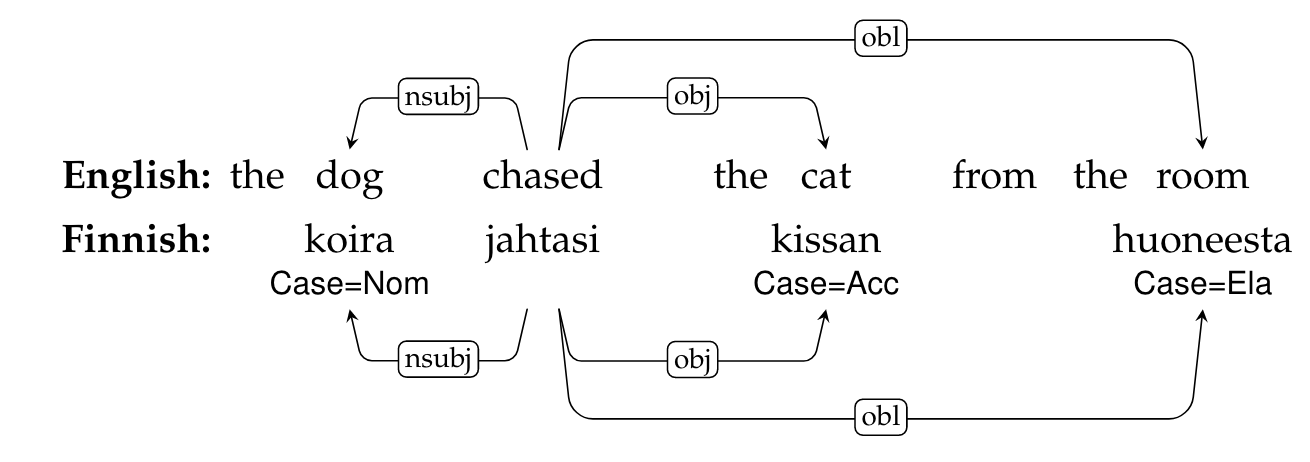
\includegraphics[width=0.85\textwidth]{figures/ud_example_sentence.png}
    \centering
    \caption{Simplified UD annotation for equivalent sentences from English (top) and Finnish (bottom) \citep{demarneffe2021}.}\label{fig:ud-example-sentence}
\end{figure}

Specifically on verbal valency, already \citet{tesniere1959} was paying attention to the cross-lingual differences in the argument structure of semantically equivalent sentences while describing his dependency grammar. Tesnière described the process of \textit{metataxis}, by which syntactic structures of one language are ``translated'' to those of another. Such a process points to the clear typological interest in valency systems, namely the mismatch between how languages encode their argument structure.

\todo{transitivity}

% focus on markedness hierarchy
In terms of possible universals that can be observed, \citet{tsunoda1981, tsunoda1985} proposed a transitivity hierarchy of verbs:
\begin{quote}
    Effective action >> Perception >> Pursuit >> Knowledge >> Feeling >> Relation
\end{quote}
The idea is that languages that encode verbs that are lower in this hierarchy as transitive verbs will encode all those above them too as transitive, with the effective action being the most prototypical transitive verb, hence most likely to be transitive in a language. This approach is further extended by \citet{malchukov2005} who used the semantic map method and proposed a two-dimensional transitivity hierarchy with the semantic map method. 

There has been some recent work from advocates of both the lexeme- and frames-based approaches on the cross-lingual alignment of their respective units of linguistic analysis. On the frames-based side, \citet{baker2020, ellsworth2021} explored the cross-lingual alignment of frames based on FrameNet; in contrast, \citet{say2014} rejected the equating of minor valency classes cross-lingually and studied how verb classes compare cross-lingually instead, seeing that as a more valid method of measuring how languages organize their verbal lexicon differently.

\chapter{Data selection}

\section{Data sources}\label{sec:data}

\subsection{Universal Dependencies}\label{subsec:data_ud}


\textbf{Universal Dependencies (UD)} is the main source of primary data used for the present study. It is designed to be a cross-linguistically consistent system for annotating morphosyntactic information within a dependency grammar framework \citep{demarneffe2021}. 

The v2 update to the UD annotation guidelines also introduced changes that intend to decrease the reliance on language-specific categories \citep{nivre2020}. Inevitably, these efforts had to be balanced against the practicality of computational efficiency but nevertheless converged in many cases with proposals by typologists, as the core principles converged with a functional typology approach. \citet{croft2017}

\begin{enumerate}
    \item UD needs to be satisfactory on linguistic analysis grounds for individual languages.
    \item UD needs to be good for linguistic typology, i.e., providing a suitable basis for bringing out cross-linguistic parallelism across languages and language families.
    \item UD must be suitable for rapid, consistent annotation by a human annotator.
    \item UD must be easily comprehended and used by a non-linguist, whether a language learner or an engineer with prosaic needs for language processing. We refer to this as seeking a \textit{habitable} design, and it leads us to favor traditional grammar notions and terminology.
    \item UD must be suitable for computer parsing with high accuracy.
    \item UD must support well downstream language understanding tasks (relation extraction, reading comprehension, machine translation, \dots).
\end{enumerate}

The \textbf{Universal Dependencies} treebanks \citep{universaldep} is the collection of cross-lingual treebanks annotated in the UD framework by an open community of more than 300 contributors. See \ref{tab:treebanks} for a table of languages available in UD v2.5, as an example.

\begin{table}[t]{}
    \centering
\begin{adjustbox}{center,scale=0.85}
\footnotesize
\renewcommand{\tabcolsep}{3pt}
    \begin{tabular}{|lrrr|lrrr|lrrr|}
    \hline
    \textbf{Language}  & \textbf{\#} & \textbf{Sents} & \textbf{Words} & \textbf{Language}  & \textbf{\#} & \textbf{Sents} & \textbf{Words} & \textbf{Language}  & \textbf{\#} & \textbf{Sents} & \textbf{Words} \\
    \hline
Afrikaans &1 &1,934 &49,276 &German &4 &208,440 &3,753,947 &Old Russian &2 &17,548 &168,522 \\
Akkadian &1 &101 &1,852 &Gothic &1 &5,401 &55,336 &Persian &1 &5,997 &152,920 \\
Amharic &1 &1,074 &10,010 &Greek &1 &2,521 &63,441 &Polish &3 &40,398 &499,392 \\
Ancient Greek &2 &30,999 &416,988 &Hebrew &1 &6,216 &161,417 &Portuguese &3 &22,443 &570,543 \\
Arabic &3 &28,402 &1,042,024 &Hindi &2 &17,647 &375,533 &Romanian &3 &25,858 &551,932 \\
Armenian &1 &2502 &52630 &Hindi English &1 &1,898 &26,909 &Russian &4 &71,183 &1,262,206 \\
Assyrian &1 &57 &453 &Hungarian &1 &1,800 &42,032 &Sanskrit &1 &230 &1,843 \\
Bambara &1 &1,026 &13,823 &Indonesian &2 &6,593 &141,823 &Scottish Gaelic &1 &2,193 &42,848 \\
Basque &1 &8,993 &121,443 &Irish &1 &1,763 &40,572 &Serbian &1 &4,384 &97,673 \\
Belarusian &1 &637 &13,325 &Italian &6 &35,481 &811,522 &Skolt S\'ami &1 &36 &321 \\
Bhojpuri &1 &254 &4,881 &Japanese &4 &67,117 &1,498,560 &Slovak &1 &10,604 &106,043 \\
Breton &1 &888 &10,054 &Karelian &1 &228 &3,094 &Slovenian &2 &11,188 &170,158 \\
Bulgarian &1 &11,138 &156,149 &Kazakh &1 &1,078 &10,536 &Spanish &3 &34,693 &1,004,443 \\
Buryat &1 &927 &10,185 &Komi Permyak &1 &49 &399 &Swedish &3 &12,269 &206,855 \\
Cantonese &1 &1,004 &13,918 &Komi Zyrian &2 &327 &3,463 &Swedish Sign Language &1 &203 &1,610 \\
Catalan &1 &16,678 &531,971 &Korean &3 &34,702 &446,996 &Swiss German &1 &100 &1,444 \\
Chinese &5 &12,449 &285,127 &Kurmanji &1 &754 &1,0260 &Tagalog &1 &55 &292 \\
Classical Chinese &1 &15,115 &74,770 &Latin &3 &41,695 &582,336 &Tamil &1 &600 &9,581 \\
Coptic &1 &1,575 &40,034 &Latvian &1 &13,643 &219,955 &Telugu &1 &1,328 &6,465 \\
Croatian &1 &9,010 &199,409 &Lithuanian &2 &3,905 &75,403 &Thai &1 &1,000 &22,322 \\
Czech &5 &127,507 &2,222,163 &Livvi &1 &125 &1,632 &Turkish &3 &9,437 &91,626 \\
Danish &1 &5,512 &100,733 &Maltese &1 &2,074 &44,162 &Ukrainian &1 &7,060 &122,091 \\
Dutch &2 &20,916 &306,503 &Marathi &1 &466 &3,849 &Upper Sorbian &1 &646 &11,196 \\
English &7 &35,791 &620,509 &Mby\'a Guaran\'i &2 &1,144 &13,089 &Urdu &1 &5,130 &138,077 \\
Erzya &1 &1,550 &15,790 &Moksha &1 &65 &561 &Uyghur &1 &3,456 &40,236 \\
Estonian &2 &32,634 &465,015 &Naija &1 &948 &12,863 &Vietnamese &1 &3,000 &43,754 \\
Faroese &1 &1,208 &10,002 &North S\'ami &1 &3,122 &26,845 &Warlpiri &1 &55 &314 \\
Finnish &3 &34,859 &377,619 &Norwegian &3 &42,869 &666,984 &Welsh &1 &956 &16,989 \\
French &7 &45,074 &1,157,171 &Old Church Slavonic &1 &6,338 &57,563 &Wolof &1 &2,107 &44,258 \\
Galician &2 &4,993 &164,385 &Old French &1 &17,678 &170,741 &Yoruba &1 &100 &2,664 \\
\hline
    \end{tabular}
\end{adjustbox}
    \caption{Languages in UD v2.5 with number of treebanks (\#), sentences (Sents) and words (Words) \citep{nivre2020}.}
    \label{tab:treebanks}
\end{table}

The thesis uses the UD v2.11 release.

In additional to the main data source of UD treebanks, additional resources will be used in the study as reference and to perform validation and evaluation of the intermediate results. As an example, the valency frames and verb classes as induced from the UD treebanks will be validated, where possible, against the expert-annotated data from \textbf{the Valency Patterns Leipzig Online Database (ValPaL)} \citep{valpal}. Other datasets will be introduced as necessary.

\section{Representing verb instances}

In the first step, the specific uses of verbs are abstracted through a feature selection process. Each instance of verb use will be represented by the morphosyntactic features of the sentence, namely only features that are considered part of valency frame encoding are included. This is in order to focus on whether semantically coherent verb classes can be induced from valency frame information alone. In selecting the features, cross-lingual differences in valency frame coding will be taken into account, e.g., whether a language uses morphological cases or word order to encode valency frame information. Word order information, although not explicitly specified in UD, should also be extracted from the dataset. An alternative approach considered is to keep manual feature selection at a minimum and to allow the clustering algorithms to weigh the features as needed.

\section{Clustering}

The clustering process after feature selection consists of two steps, but the clustering algorithms used need not be the same. The first is the automatic induction of valency frames in a language given the selected features and the second is the clustering of verbs, represented by their distribution over the valency frames, into verb classes. Since unsupervised clustering will be used, the number of valency frames and the number of verb classes cannot be assumed \textit{a priori}. This requires either using algorithms that do not require a predefined number of clusters (e.g., Ward clustering), or experimenting with cluster sizes with each language (cf. \cite{schulteimwalde2006}, which used the k-means algorithm with a predefined the gold standard number). Due to the lack the gold standard for many of the languages to be experimented on, the former seems preferable. A bottom-up agglomerative clustering method will also be favored over top-down methods.

Given the relative low dimensionality of hand-selected features, complex clustering algorithms are not anticipated to be necessary. Nevertheless, more modern clustering algorithms should also be investigated \citep{xu2015a}. Given the two levels of clustering, one method to be considered for the verb class induction is the Hierarchical Dirichlet process, which is particularly suited for clustering grouped data (cf. \citet{parisien2010}, Fig.~\ref{fig:parisien2010}, where a Hierarchical Dirichlet process was extended to account for diathesis alternations).
·
\begin{figure}
    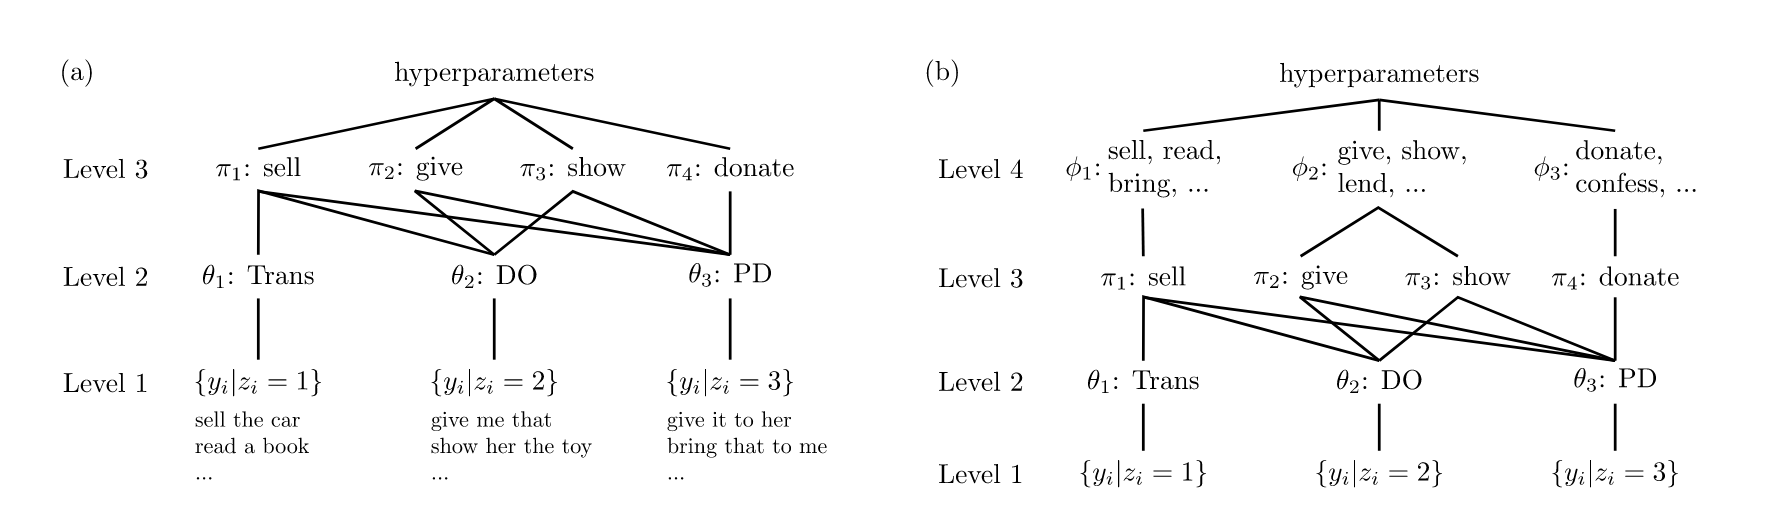
\includegraphics[width=\textwidth]{figures/verb_alternation_classes.png}
    \centering
    \caption{(a) Model 1, a Hierarchical Dirichlet Process applied to learning verb argument structure constructions. (b) Model 2,
    an extension of Model 1 to learn verb alternation classes.}\label{fig:parisien2010}
\end{figure}

\section{Cross-lingual verb sense alignment}

A cross-lingual aligned list of counterpart verbs will be needed to compare the verb classes. The easiest way to do this is likely through existing cross-lingual word lists such as LanguageNet, part of the PanLex project \citep{kamholz2014}. However, multilingual word embeddings and induction of a cross-lingual verbal lexicon could be considered as another option should the existing resources prove insufficient.

\section{Information theory metrics}

The specific metrics to be used on the results will have to be determined in combination with the decisions to be made in the experiments such as the number of the language studied and whether parallel or non-parallel datasets are used. Preliminarily, however, information theory metrics modeled on those used by \citet{say2014} are considered, specifically an internal complexity metric measuring the entropy of the distribution of verbs among valency classes and a similarity metric based on mutual information measuring the similarity / dissimilarity between valency systems of two or more languages.
\chapter{Comparing transitivity across languages}\label{chapter:transitivity}

\section{From transitivity categories to transitivity ratios}

It is logical when doing cross-linguistic comparison to start with simpler metrics and features before developing to more complex ones. On the one hand, it is true that regardless of how we approach the task of verb classification, i.e., to categorize the verbs of a language into verb classes according to their syntacto-semantic properties and behavior, we would expect to arrive at fine-grained verb classes à la \citet{levin1993} in the end. On the other hand, such an expectation does not render obsolete the more basic distinctions like that of verb \textit{transitivity}. In part, this is due to their utility as convenient starting points of comparison for verbs within a language, but their simplicity also translates to being more cross-lingually valid bases of typological comparison. 

This first experiment deals with metrics of \textit{transitivity}, i.e., the ability of a verb to take one or more objects. It is surely a more familiar and intuitive concept as compared to the finer-grained metrics of valency to follow in the experiments in the next chapter. In traditional grammars, a basic binary distinction is made between \textit{intransitive} verbs, which take only a subject and no objects and \textit{transitive} verbs, which take one or more objects. Additional categories, some overlapping, make finer distinctions, such as \textit{ditransitive} verbs (those taking two objects), \textit{ambitransitive} verbs (those that can be used both transitively and intransitively), etc.

I focus here on the simple distinction between transitive and intransitive verbs, but, hewing to a functional and quantitative outlook, find that binary categories do not sufficiently capture the nuances of verb use. An example illustrating why comes from the study of near-synonyms: \citep{biber1998}, an early corpus linguistics study, compares the English verbs \textit{begin} and \textit{start} in the British National Corpus (BNC). At first glance, English appears to have provided us with two verbs that are not only semantically synonymous but share valency properties as well, as they can both be used in transitive and intransitive constructions:

\begin{exe}
\ex\label{example-begin_start}
  \begin{xlist}
  \ex{I had better issue a survival kit before we \textit{start}/\textit{begin}.\\ \strut\hfill \textbf{intransitive}}
  \ex{Then they \textit{started}/\textit{began} the quota system.\\ \strut\hfill \textbf{transitive with noun phrase}}
  \ex{They'd \textit{started}/\textit{begun} leaving before I arrived.\\ \strut\hfill \textbf{transitive with \textit{-ing} clause}}
  \ex{One of the wheels had \textit{started}/\textit{begun} to wobble.\\ \strut\hfill \textbf{transitive with \textit{to} clause}}
  \end{xlist}
\end{exe}

This however belies their different usage patterns as observed in the BNC: while both uses are clearly grammatical for both verbs, \textit{begin} is used more often in a transitive frame than \textit{start} across different genres in the BNC: in fiction, 78\% of \textit{begin} occurrences (196/250) are with various transitive patterns vs. only 60\% for \textit{start} (149/250); transitive uses are less frequent in academic texts in general but the observation of relatively higher transitivity for \textit{begin} still holds (57\% vs. 36\%, or 110/192 vs. 51/142).

To capture such differences in levels of transitivity, I propose measuring \textbf{transitivity ratios} based on language corpora, defined as the percentage of verb instances that are transitive. The verbs of a language can then be thought of as on a spectrum of transitivity, with strictly intransitive verbs on the one end, strictly transitive verbs on the opposite end, and all other verbs\footnote{Note that not all of them are ambitransitive verbs, as the approach here is only concerned with the surface realization of transitivity. In particular, this means instances of pro-drop of objects are counted as intransitive, where some would argument for a null object analysis instead.} somewhere in between.

\section{Experiment 1:Token-level transitivity ratios}\label{sec:exp1}
\subsection{Calculating transitivity ratio from UD}

Necessarily then, and in contrast with transitivity categories, any values are calculated on an \textit{ad hoc} basis in a given corpus. Unless we expect the corpus to be a representative sample of all language use in that language, which is certainly not the case for the UD corpora used here, the absolute values of these ratios at a lexeme-level cannot be directly interpreted. Instead, intralinguistic analysis will take the form of analyzing the distribution of verbs according to their observed transitivity ratios. I take on an additional assumption, that the corpus would reflect the general tendency towards (in-)transitivity of the language, if too piecemeal for individual verbs, which justifies the cross-lingual comparison of transitivity ratios at a token-level as well.

The UD annotation scheme facilitates the investigation of transitivity at lexeme- and token-levels, as the relevant dependency relations \textsc{nsubj} and \textsc{obj} mark respectively the first and second core arguments of a verb with their typical syntactic roles as subject and object. This is defined without respect to specific cases (even though typically the nominative and the accusative in languages with a case system) or semantic roles (even though they would typically be the proto-agent and the proto-patient) in an effort to avoid \textit{a priori} categories to the extent possible. The renaming of the \textsc{dobj} relation to \textsc{obj}, among the changes introduced by UD v2 \citep{nivre2020}, reflects the same laudable effort.

Despite the typologically sound UD dependency relation annotations, arriving at a clear definition of transitivity ratio in the UD context is still not trivial upon close examination. In fact, I consider four different definitions of a quantitative transitivity ratio within the UD annotation scheme here:

\begin{enumerate}
    \item the ratio of verb instances with both \textsc{nsubj} and \textsc{obj} dependents, as compared to verb instances with an \textsc{nsubj} dependent
    \item the ratio of verb instances with an \textsc{obj} dependent, as compared to verb instances with an \textsc{nsubj} dependent
    \item the ratio of verb instances with an \textsc{obj} dependent, as compared to all verb instances
    \item the ratio of verb instances with an \textsc{obj} dependent, as compared to verb instances with either an \textsc{nsubj} or an \textsc{obj} dependent
\end{enumerate}

Def. 1 is an attempt at enforcing a definition of the transitive object as the \textit{second} core argument of the verb by excluding from calculation instances where the first core argument (i.e., subject) is not realized. This turns out counterproductive for two reasons. Firstly, this does not sit well with the core definition on transitivity, as instances of verb use where the subject is not expressed should not count against the fact that the verb is taking a transitive object; secondly, this is undesirable in practice when accounting for typological variations, as the metric would be biased against pro-drop languages that drops subject pronouns more often than objects such as Spanish.

Revising def. 1 and dropping the requirement in the numerator for verbs to have an \textsc{nsubj} dependent gives us def. 2. However, this is not sufficient, as the opposite problem surfaces, where subject-dropping languages are likely to have a smaller denominator, resulting in a high transitivity ratio that is not representative. Def. 3 drops the \textsc{nsubj} requirement from the denominator as well. This still faces problems, as verb instances where both subject and object are dropped would affect the denominator, and such usage, e.g., non-predicative usage of verbs, is unlikely to be equally frequent in different languages and would therefore interfere with the cross-lingual comparability of our transitivity ratio focusing on argument structure of verb predicates. Taking all these potential drawbacks into consideration, we arrive at def. 4 with the number of verb instances with either an \textsc{nsubj} or an \textsc{obj} dependent in the denominator. 

\begin{table}[ht]
    \centering
    \begin{tabularx}{0.5\textwidth}{cX}
    {\#} & \textbf{Definition} \\
    \hline
    1&$[+\textsc{nsubj}, +\textsc{obj}]/ [+\textsc{subj}]$ \\
    2&$[+\textsc{obj}] / [+\textsc{nsubj}]$  \\
    3&$[+\textsc{obj}] / [\pm\textsc{nsubj}, \pm\textsc{obj}]$\\
    4&$[+\textsc{obj}] / [+\textsc{nsubj}] \text{ or } [+\textsc{obj}]$
    \end{tabularx}
    \caption{Potential definitions of transitivity ratio considered in §\ref{sec:exp1}, represented with feature matrices}\label{tab:transitivity-defs}
\end{table} 

While there is a strong case for Def. 4 being the most principled definition, I nevertheless implement all four definitions in this experiment to empirically verify the intuitions. They are also represented with feature matrices in Tab.~\ref{tab:transitivity-defs} for quick reference.

\subsection{Transitivity ratios and the lexicon}\label{subsec:transitivity-lexicon}

Transitivity ratio statistics for each verb lexeme based on the definitions are first compiled. From there, per-language statistics that will become the basis for our cross-lingual comparison are computed: I calculate the lexeme-level and token-level transitivity ratios for each language, respectively the arithmetic mean of the lexeme transitivity ratios and the mean of lexeme transitivity ratios weighted by the frequency of the lexeme. In addition to the transitivity ratio metrics, an additional metric, percentage of transitive verbs, i.e., the percentage of verbs in the observed lexicon that are not strictly intransitive (defined as never observed to take an \textsc{obj}), is calculated for comparison purposes, as it should correspond better with the traditional binary distinction between transitive and intransitive verbs.

I perform the experiment on the selected subset of UD data as described in §\ref{sec:data_selection}. For the analysis, I include only languages with at least 100 observed verb lexemes (56 out of 79 languages); the full results from the experiments can be found in the accompanying data and appendices. 

\begin{table}[ht]{}
    \centering
    \small
    \begin{tabularx}{\textwidth}{lXXX}
      \toprule
      def. & lexeme tr.,\newline token tr. & tr. verb \%,\newline lexeme tr. & tr. verb \%,\newline token tr. \\
      \midrule
      1 & $\rho(54)=.83, p=.000$ & $\rho(54)=.61, p=.000$ & $\rho(54)=.70, p=.000$ \\
      2 & $\rho(54)=.81, p=.000$ & $\rho(54)=-.17, p=.221$ & $\rho(54)=-.03, p=.817$ \\
      3 & $\rho(54)=.77, p=.000$ & $\rho(54)=.64, p=.000$ & $\rho(54)=.73, p=.000$ \\
      4 & $\rho(54)=.87, p=.000$ & $\rho(54)=.61, p=.000$ & $\rho(54)=.61, p=.000$ \\
      \bottomrule
    \end{tabularx}
    \caption{Spearman's rank correlation between the transitivity metrics}\label{tab:transitivity_spearmanr} 
\end{table}  

To compare between the different definitions of transitivity, we compute Spearman's rank correlations between the lexeme- and token-level means of transitivity ratios according to each of our four definitions, as well as between the transitive verb percentage and each of them. The correlation statistics are listed in Tab.~\ref{tab:transitivity_spearmanr}. We observe overall strong correlations between the mean transitivity ratios at lexeme- and token-levels for all four definitions, with the highest observed for definition 4 ($\rho(54)=.87, p=.000$) and lowest observed for definition 3 ($\rho(54)=.77, p=.000$). The strong correlation is not surprising as we have no reason to expect the more frequent verbs to behave differently from the less frequent verbs with regard to transitivity ratios. This can also be confirmed by correlation tests between verb frequency and verb transitivity ratios for each language, which show no strong correlation.

The correlation statistics between the transitive verb percentages and the transitivity ratios are slightly more revealing. If nothing else, they help us eliminate definition 2 from the competition as it shows no statistically significant correlation ($\rho(54)=-.17, p=.221$ for lexeme-level transitivity ratios and $\rho(54)=-.03, p=.817$ for token-level) while strong correlations are observed for all three other definitions (see Tab.~\ref{tab:transitivity_spearmanr}).

In the absence of a practical reason based on correlation statistics to select a definition among the remaining three over the others, the rest of the analysis uses def. 4, which I have considered \textit{a priori} to be the most principled. Further intralinguistic analyses are done by plotting histograms of the distributions of verbs among the transitivity ratios in different languages, as shown in Fig.~\ref{fig:verb_dist_transitivity}.

\begin{sidewaysfigure}[ht]
  \centering
  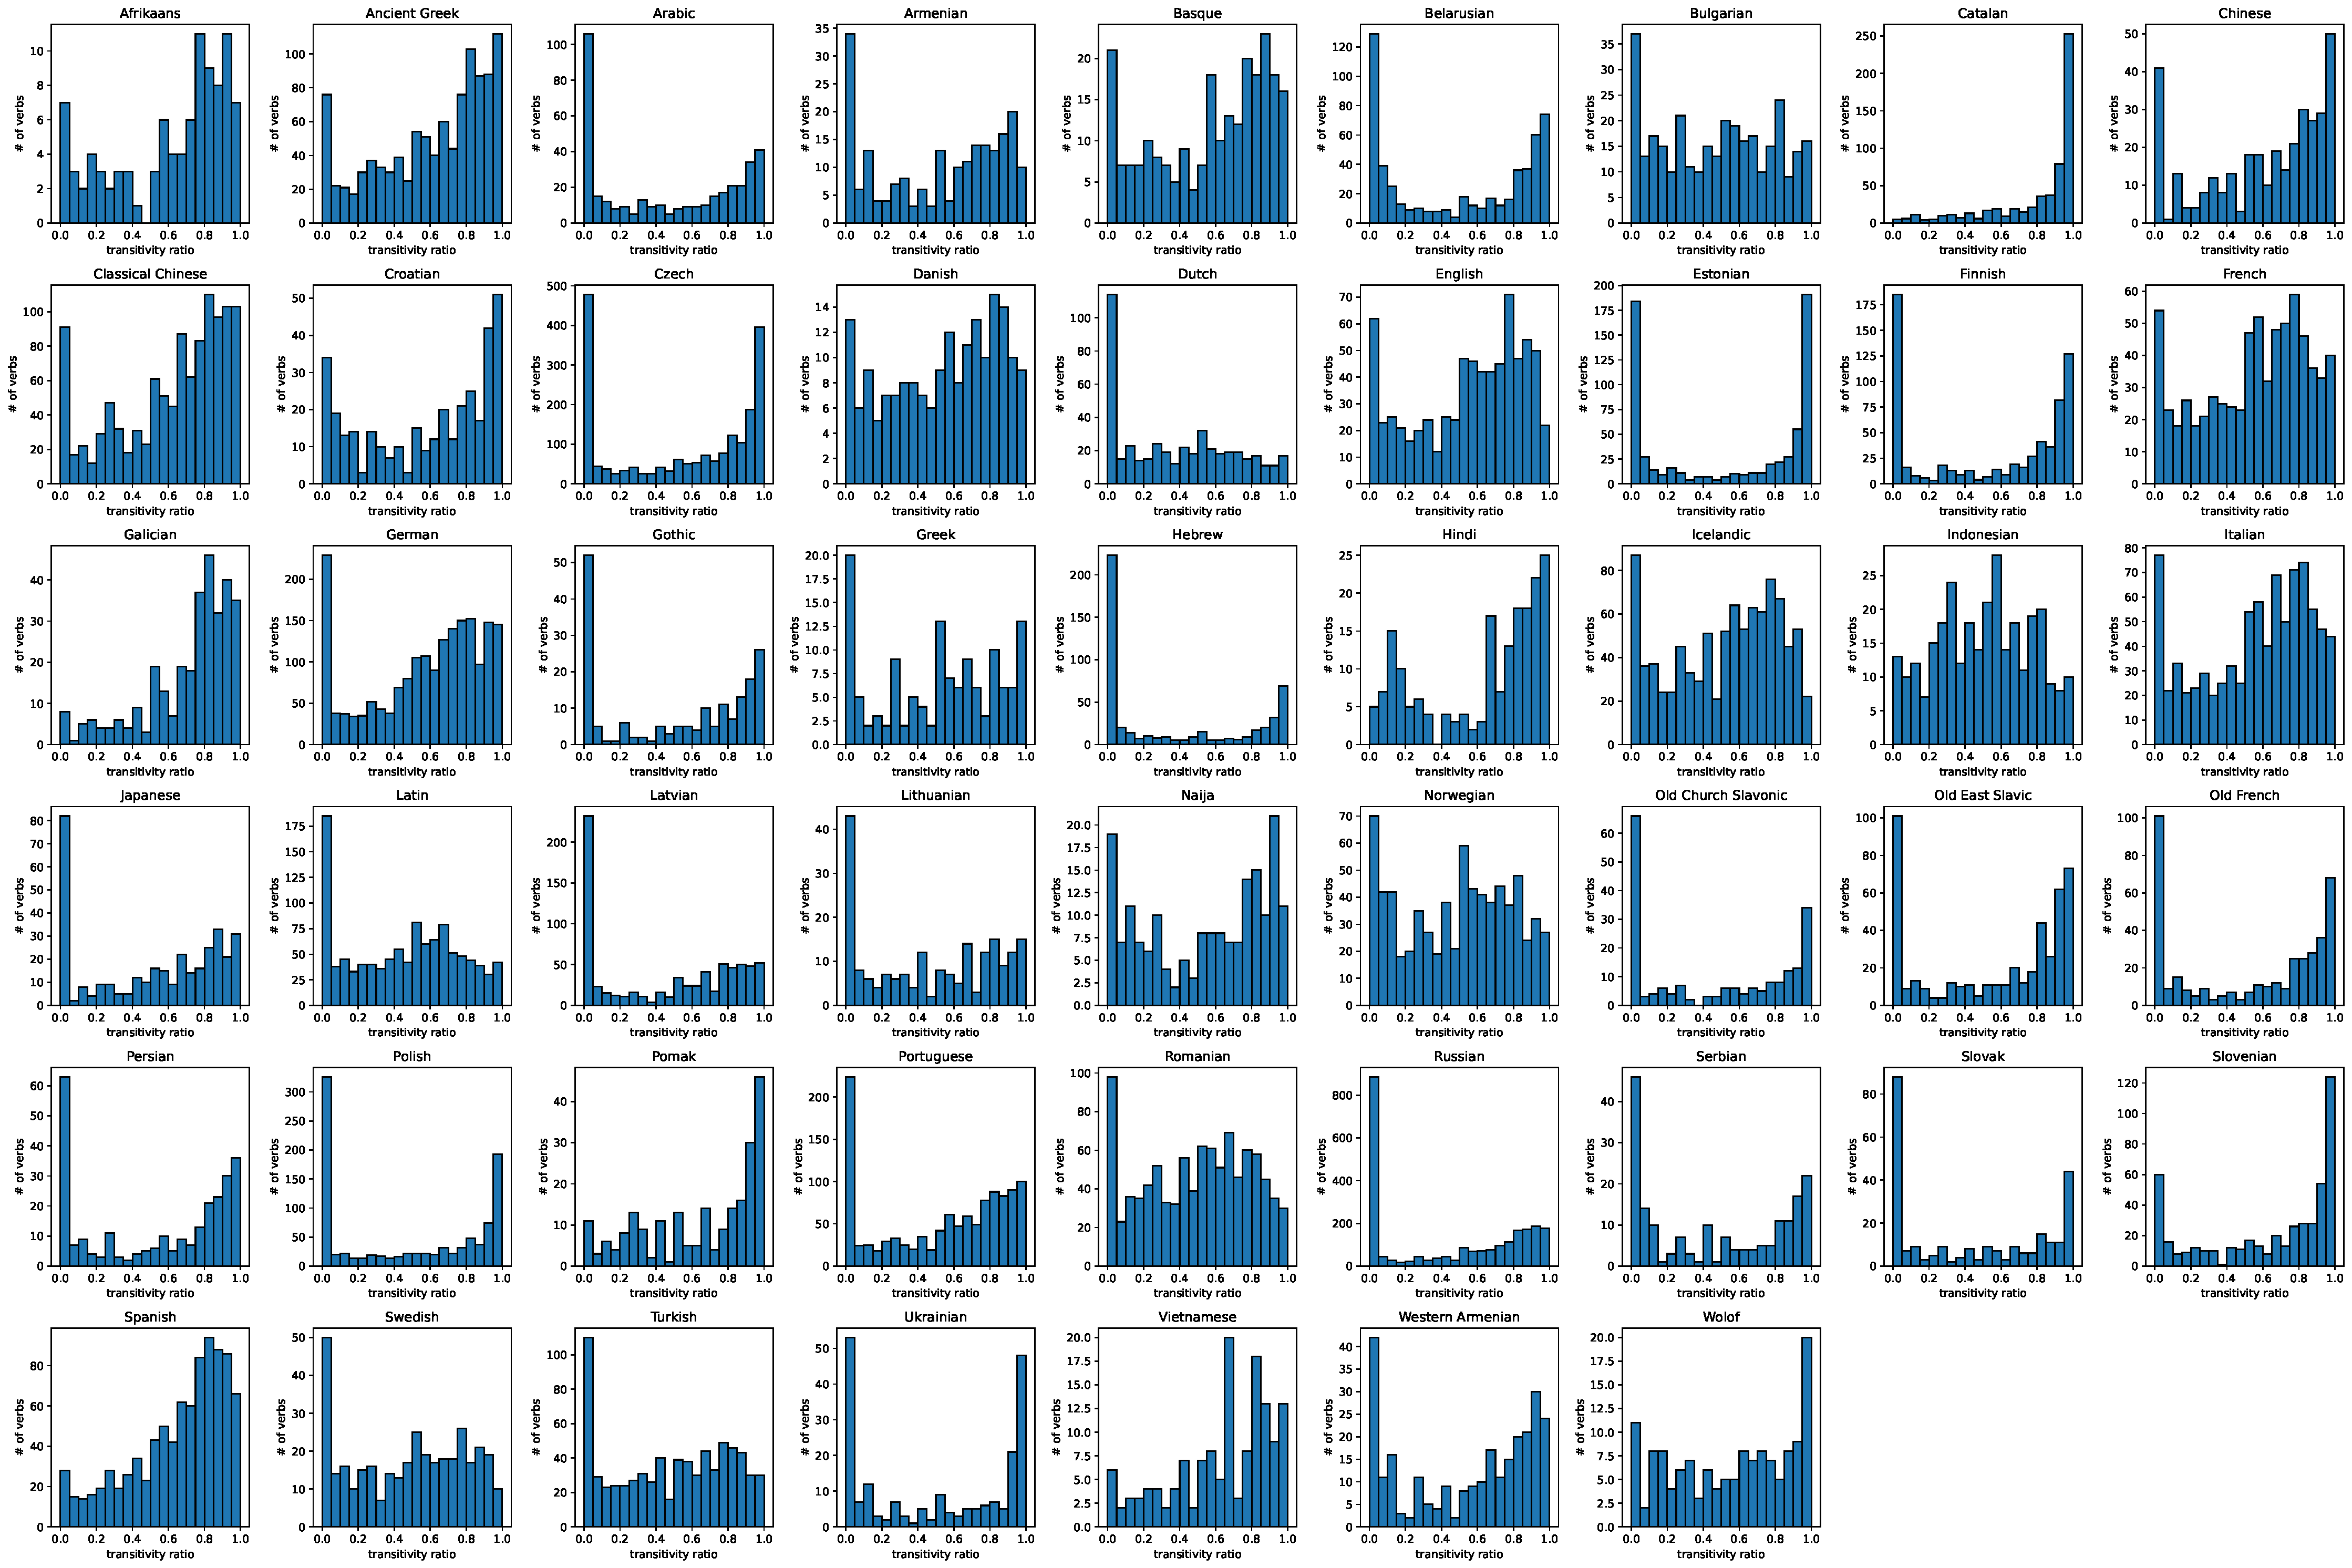
\includegraphics[width=\textwidth]{figures/verb_dist_by_transitivity.pdf}
  \caption{Histograms showing the binned distributions of verbs according to their transitivity ratio in different languages}
  \label{fig:verb_dist_transitivity}
\end{sidewaysfigure}

Most distributions are bimodal with peak at both ends, which supports the overall cross-lingual validity of a binary conception of transitivity. But exceptions abound as well, among others Indonesian (unimodal with peak in the middle), Catalan, Galician, Spanish (unimodal with peak on right). And even between the bimodal distributions, they are notably rarely symmetric, with differing levels of skew towards either end. 

\subsection{Genetic and areal patterns in transitivity}

\begin{table}[ht]
    \centering
    \small
    \begin{subtable}[c]{\textwidth}
      \centering
      \begin{tabular}{lrr|lrr}
        \toprule
        Language & \# Verbs & Tr. verb \% & Language & \# Verbs & Tr. verb \% \\
        \midrule
        Catalan & 628 & 99.2\% & Maltese & 78 & 55.1\% \\
        Galician & 341 & 97.7\% & Hebrew & 536 & 58.4\% \\
        Urdu & 69 & 97.1\% & Hungarian & 73 & 64.4\% \\
        Hindi & 207 & 97.1\% & Russian & 2583 & 65.0\% \\
        Spanish & 948 & 96.9\% & Slovak & 284 & 66.5\% \\
        Indonesian & 330 & 96.7\% & Uyghur & 93 & 66.7\% \\
        Vietnamese & 156 & 95.5\% & Coptic & 128 & 68.0\% \\
        French & 735 & 94.8\% & Old Church Slavonic & 223 & 68.6\% \\
        Gheg & 50 & 94.0\% & Polish & 1080 & 68.8\% \\
        Danish & 212 & 93.9\% & Bambara & 50 & 70.0\% \\
        English & 773 & 93.4\% & Erzya & 87 & 70.1\% \\
        Afrikaans & 119 & 93.3\% & Latvian & 794 & 71.2\% \\
        Norwegian & 765 & 92.9\% & Gothic & 201 & 73.1\% \\
        Basque & 255 & 92.9\% & Old French & 444 & 74.1\% \\
        Ancient Greek & 1127 & 92.7\% & Faroese & 117 & 74.4\% \\
        \dots & \dots & \dots & \dots & \dots & \dots \\
        \bottomrule
      \end{tabular}
      \caption{by transitive verb percentage}
      \label{tab:most_tr_by_verb_percentage}
    \end{subtable}\\
    \begin{subtable}[c]{\textwidth}
      \centering
      \begin{tabular}{lrr|lrr}
        \toprule
        Language & \# Verbs & Token tr. & Language & \# Verbs & Token tr. \\
        \midrule
        Akkadian & 76 & 75.9\% & Scottish Gaelic & 53 & 16.2\% \\
        Catalan & 628 & 75.9\% & Irish & 108 & 30.8\% \\
        Galician & 341 & 70.5\% & Maltese & 78 & 31.7\% \\
        Afrikaans & 119 & 65.3\% & Faroese & 117 & 32.6\% \\
        Urdu & 69 & 65.2\% & Japanese & 395 & 33.4\% \\
        Gheg & 50 & 64.8\% & Hebrew & 536 & 33.5\% \\
        Vietnamese & 156 & 64.8\% & Polish & 1080 & 34.0\% \\
        Thai & 77 & 64.7\% & Uyghur & 93 & 34.1\% \\
        Classical Chinese & 1192 & 63.8\% & Erzya & 87 & 36.0\% \\
        Pomak & 244 & 62.1\% & Russian & 2583 & 37.4\% \\
        Spanish & 948 & 61.1\% & Dutch & 497 & 37.5\% \\
        Hindi & 207 & 60.8\% & Latvian & 794 & 37.8\% \\
        Chinese & 380 & 60.7\% & North Sami & 76 & 38.2\% \\
        Xibe & 74 & 58.8\% & Serbian & 214 & 38.4\% \\
        Ancient Greek & 1127 & 58.5\% & Arabic & 407 & 39.7\% \\
        \dots & \dots & \dots & \dots & \dots & \dots \\
        \bottomrule
      \end{tabular}
      \caption{by token-level transitivity ratio}
      \label{tab:most_tr_by_token_mean}
    \end{subtable}
    \caption{Most and least transitive languages by different metrics}
    \label{tab:most_tr_languages}
  \end{table}

Tab.~\ref{tab:most_tr_by_verb_percentage} and \ref{tab:most_tr_by_token_mean} list the most and least `transitive' languages in our study, respectively according to the transitive verb percentage and the token-level transitivity ratio. Recall that token-level transitivity ratios are favored over lexeme-level ones for cross-lingual comparison.

Among the most transitive languages are Romance (Catalan, Spanish, French, Galician) and Germanic (German, Norwegian, English, Danish) languages of Europe, Sinitic languages (Chinese, Classical Chinese, particularly when measured by token-level transitivity ratio), Indonesian, Hindi. On the opposite end of the spectrum are Hebrew, Irish, Japanese, as well as Baltic (Lithuanian, Latvian) and Slavic (Slovak, Russian, Polish) languages, which have the lowest transitivity ratios.

\begin{sidewaysfigure}[ht]
  \centering
  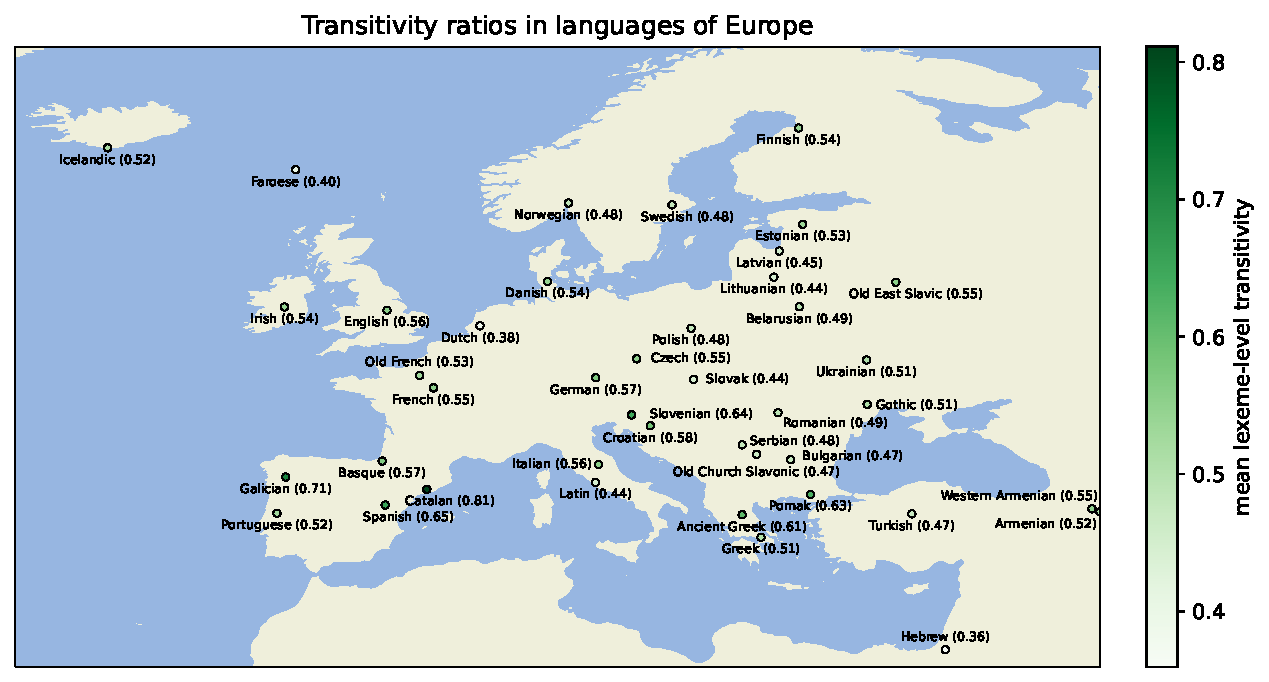
\includegraphics[width=\textwidth]{figures/transitivity_europe.pdf}
  \caption{Mean transitivity ratios in languages of Europe}
  \label{fig:transitivity_europe}
\end{sidewaysfigure}

To look at any potential areal patterns in transitivity, the token-level transitivity ratio results for European languages are also mapped in Fig.~\ref{fig:transitivity_europe}. (A less Eurocentric study of areal patterns is unfortunately difficult for the lack of enough language samples in the UD.) A particularly high transitivity area can be observed in the Iberian peninsular as well as another relatively high transitivity area in the Balkans, in contrast to eastern and northern Europe with lower transitivity.

Where the languages overlap, these observations match well with those from \citet{say2014}'s survey of transitivity in European languages (as measured by the percentage of verbs that are transitive from a fixed list), who observed high transitivity areas in western Europe except Irish and south-western Balkans, and a corresponding low transitivity area in eastern Europe.

% Dutch appears to be a special case in several ways. \todo{case study: Dutch - divergence btwn two metrics, maybe due to ergative verbs? and diff btwn Dutch vs Afrikanns - significant grammatical differences?}

% diff between tr. verb -> token-level tr. ratio reflects also the fact that tr. verbs can often be used intransitively
% how "free" a language is to use tr. verb  intr./vice versa is another interesting further study 

\chapter{Entropy-based measures of verbal valency}\label{chapter:entropy}

While the previous chapter has demonstrated that corpus-based transitivity ratios can serve as a useful basis for typological comparison, it is still is a relatively simple metric that captures one aspect of verbal valency. Put another way, transitivity ratio can be seen as a subset of the scope needed for a more holistic investigation into verbal valency, as it concerns only one type of verb dependent, i.e., the object, and one feature of this dependent, i.e., its presence or absence. 

This chapter undertakes to expand the scope of investigation accordingly, to cover both more verb dependent types and more features of them. Instead of performing exhaustive comparisons on each individual feature of each dependent, the focus is on the variability of \textit{valency frame alternations} (also called diathesis alternations), i.e., the range of valency frames in which a verb appears and how likely it is to appear with each frame. New entropy-based measures of verbal valency are proposed and tested in conjunction with hypotheses about the structure of valency systems.

The sections are organized as follows: §\ref{sec:entropy-background} provides a brief background on cognitive and psycholinguistic perspectives on language structure, in particular relating to the frequency effect and valency frame alternation, which motivate the hypotheses tested in the experiments; in §\ref{sec:valency-frame-encoding}, the feature selection and extraction procedures of valency frame encoding from UD are described, as they form the basis for the experiments in this chapter. 

Four experiments are then presented: Experiment 2 (§\ref{sec:exp2-valency-frame-entropy}) uses joint entropy to define the valency frame entropy measure and tests its correlation with verb frequency; Experiment 3 (§\ref{sec:exp3-ablation}) examines cross-lingual variations in how languages encode the valency frames, by means of an ablation study using conditional entropy to assess the contribution of word order and case marking to the overall valency frame entropy; Experiment 4 (§\ref{sec:exp4-verb-entropy}) takes a frame-based approach and, in symmetry to Experiment 2, calculates the correlation between verb entropy and frame frequency.

% Experiment 4 (§\ref{sec:exp4-verb-specificity}) uses conditional entropy measure and seeks to quantitatively verify the verb specificity test that is used to distinguish core and non-core dependents (complements and adjuncts); 

\section{Valency frame, frequency and the efficient organization of the lexicon}\label{sec:entropy-background}

Cognitive linguists and typologists have increasingly sought to integrate the two approaches in the same functionalist research paradigm \citep{croft2016}. Among others is research that seeks to examine and explain language-internal and cross-linguistic features of human languages through the lens of communicative efficiency, at various levels including the lexicon, syntax and morphology (see \citealp{gibson2019} for a survey). 

An early example where efficiency is used to explain phenomena in human languages is the work of George Kingsley \citet{zipf1935,zipf1949}. He first studied what is now known as Zipf's law, the empirical observation of the negative correlation between word length and frequency, that ``the magnitude of words tends, on the whole, [stands] in an inverse (not necessarily proportionate) relationship to the number of occurrences'', and sought to explain it through the principle of least effort.

Frequency is a particularly frequent lens through which the lexicon is examined and the correlation between frequency and other features often subjects of hypotheses. Its importance has been further underlined by psycholinguistic studies which show a consistent ``frequency effect'' for both open and closed class word \citep{segui1982,marslen-wilson1990}, where more frequently occurring words have a higher resting activation, making their lexical retrieval easier. That the most frequent lexical items are also more likely to be associated with irregularity is not surprising. This correlation between frequency and irregularity has most often been hypothesized and studied for morphology \citet{wu2019}. \citet{bybee1998} considers lexicon from a learnability perspective and postulates a trade-off in the lexical memory that ``being easier to access, they are less likely to be replaced by regular formations''. 

When it comes to verbal valency, psycholinguistic studies have also consistently shown the effect of semantic and syntactic attributes of the verb on online sentence processing \citep{shapiro1987,collina2001}. Results differ on whether subcategorization (syntactic), thematic frames (semantic) or both have an effect on lexical processing. \citet{shapiro1987} reported that RTs for lexical decisions increased as the function of the number of thematic options instead of subcategorization options. In contrast, \citet{shetreet2007} reported on an fMRI study on Hebrew speakers, shows that the number of options in terms of subcategorization and thematic frames is better correlated to activity in the cortical areas that are associated with linguistic processing, as opposed to the number of complements or thematic frames.

In the following experiments, I will test a few hypotheses between frequency metrics on the one hand and entropy metrics on the other hand and show that, regardless of the theoretical stance, how a language structures its valency system reflects trade-offs predicted by considerations of efficiency and learnability.

\section{Extracting valency frame encoding from UD}\label{sec:valency-frame-encoding}

As briefly discussed in the data chapter, UD annotations make available a range of information related to the morphosyntactic encoding of valency frame, beyond the transitivity information that we have already used. The following experiments in this chapter make use of this for a more fine-grained characterization of the variation in valency frame encoding for different verbs using entropy-based measures. To do so, \textbf{valency frame encoding}, i.e., the scope of the morphosyntactic features that compose a valency frame, must first be extracted from the UD annotations so that variation patterns can be consistently captured. The extraction procedures are described in this section.
\subsection{Dependency relations}

\begin{table}
  \centering
  \begin{tabular}{ll}
    \toprule
    \textbf{UD label} & \textbf{Dependent} \\
    \midrule
    \multicolumn{2}{l}{\textit{core arguments}} \\
    \textsc{nsubj} & nominal subject \\
    \textsc{obj} & object \\
    \textsc{csubj} & clausal subject \\
    \textsc{ccomp} & clausal complement \\
    \textsc{xcomp}   & open clausal complement \\
    \textsc{iobj} & indirect object \\
    \midrule
    \multicolumn{2}{l}{\textit{non-core dependents}} \\
    \textsc{obl} & oblique nominal \\
    \textsc{expl} & expletive \\
    \textsc{advmod} & adverbial modifier \\
    \textsc{advcl} & adverbial clause modifier \\
    \bottomrule
  \end{tabular}
  \caption{UD dependency relation labels included in valency frame extraction}\label{tab:ud-dependent-labels}
\end{table}

From UD annotations, I start by determining which dependency relations of the verb to include as part of the valency frame. The distinction between argument (complement) and adjunct is a well-established one in linguistics, the former being obligatory and the latter optional. UD annotations schema \citep{demarneffe2014}, including in the up-to-date v2 guidelines\footnote{\url{https://universaldependencies.org/u/dep/}, archived on 30-07-2023 at \url{https://web.archive.org/web/20230730071650/https://universaldependencies.org/u/dep/}}, makes the distinction between \textit{core arguments} (i.e. subject and object) and everything else (called \textit{non-core dependents}) instead. All core arguments as classified by UD are included in the analysis. This includes nominal dependents (\textit{nominal subject}, \textit{object}, \textit{indirect object}) as well as clausal dependents (\textit{clausal subject}, \textit{clausal complement}, \textit{clausal complement}). 

As the non-core dependents still include arguments which complete the verbal meaning (in particular, \textit{obliques}), and, as a priori distinctions between arguments and adjuncts are unnecessary for this study, possibly even counterproductive, given the quantitative experiment design, a subset of non-core dependents are included as well, namely oblique nominal, expletive, adverbial modifier and adverbial clause modifier. Other non-core dependents from UD are excluded for various reasons, either due to relatively low cross-lingual uniformity in interpretation (e.g., \textit{dislocated element}), or due to being suprasentential elements (e.g. \textit{vocative}, \textit{discourse element}). Tab.~\ref{tab:ud-dependent-labels} shows the list of dependents included in the study.

It is important to note that the basis of cross-linguistic comparison will be the taxonomy of the dependencies and the valency frames they compose. The validity of the study is therefore predicated on the cross-lingual validity of the UD relations, which, while certainly not perfect, is as good as one can do, given that UD is designed with it in mind, but otherwise agnostic as far as linguistic theory is concerned. In other words, it does not matter whether the UD category \textit{indirect object} corresponds to the traditional grammatical category of indirect object, in so far as the cross-linguistically dependents serving equivalent functions are consistently annotated.

\subsection{Feature extraction}

For each of dependent relations in Tab.~\ref{tab:ud-dependent-labels}, I extract three features: (1) the presence or absence of dependency relations attached to a verb token, (2) the relative word order information, whether specific dependents precede or follow the head verb, and (3) morphological case marking on the dependents, if any. In terms of implementation, the valency frame of each verb token is represented in a feature array encoding the three types of feature with the size of $3\times$ the number of dependents. Any verbs that share the same feature array are said to have the same valency frame.

\section{Experiment 2: Frequency correlation with valency frame entropy}\label{sec:exp2-valency-frame-entropy}

\subsection{Introduction}
This experiment introduces a valency frame entropy metric, conditioned on the verb, that measures the average amount of surprisal, i.e., uncertainty, associated with the valency frame alternation for a verb, and hypothesize a positive correlation between a verb's frequency and the valency frame entropy conditioned on it that should hold across languages. In other words, the more frequent a verb is, the more information content one can expect on average from its valency frames.

A learnability perspective on the lexicon provides one motivation behind the hypothesis. Taking the view that the lexicon is acquired from linguistic experience, more exposure to and access of the more frequent words leads to higher resting activation (cf. \citealp*{bybee1998}), therefore allowing for more complexity or uncertainty being retained in the lexicon. This is analogous to the correlation between word frequency and irregularity in morphological patterns. However, whereas morphological irregularity is a purely formal feature, the choice of valency frame often entails a semantic choice as well.

If viewed from a production and comprehension perspective, the hypothesis is also potentially relevant to the Uniform Information Density (UID) hypothesis \citep{fenk1980,levy2006}, which posits that language speakers prefer a more even distribution of surprisal values across utterances in order to maximize but not overload the capacity of the communication channel. Less frequent verbs would already have high surprisal, having high entropy in the valency frames associated with it is undesirable due to channel capacity constraints. I note, however, that UID hypothesis has mostly focused on surprisal at a token/phoneme-level. This is the case for the verb in question, but the valency entropy measures aspects of the morphosyntax of the sentence instead and requires a clearer formulation of the relationship between the frames and the tokens that compose it. Nevertheless, at a high level the hypothesis here is congruent what is expected given the UID hypothesis.

\subsection{Methodology}

Let $X_1, X_2,\ldots,X_n$ be discrete random variables where each $X_k$ represents a UD dependency relation (e.g., \textsc{nsubj}, \textsc{obj}, \ldots). These variables have corresponding sample spaces $\mathcal{X}_1, \mathcal{X}_2, \ldots, \mathcal{X}_n$, which represent the possible outcomes of each variable with regard to its presence, linearized order, and any case information. Additionally, let there be a variable $V$ that represents the choice of a verb from the lexicon $\mathcal{V}$. 

The entropy of each dependency relation given a specific verb $v \in \mathcal{V}$ quantifies the average surprisal associated with that dependency relation. The \textbf{dependency relation entropy} for  $X_k$ is defined as:

\begin{equation*}
  H(X_{k}|V=v)=
  -\sum\limits_{x_{k}\in{}\mathcal{X}_{k}}{P(x_{k}|V=v)\log_{2}{P(x_{k}|V=v)}}  
\end{equation*}

Here, $P(x_k | V = v)$ represents the conditional probability of the outcome $x_k$ of the dependency relation $X_k$ given that the verb variable $V$ takes on the value $v$. The entropy of $X_k$ is calculated by summing the products of these probabilities with their logarithms (base 2) taken, each corresponding to a possible outcome $x_k$.

The \textbf{valency frame entropy} is formalized as the joint entropy of the relevant UD dependency relations, i.e., number of bits needed to encode the entire valency frame. Denoted as $H_{\text{joint}}(X_1, X_2, \ldots, X_n | V = v)$, it quantifies the uncertainty associated with the combined set of random variables $X_1, X_2, \ldots, X_n$, again given a specific value $v$ for the verb variable $V$. This is defined as:

\begin{equation*}
\begin{split}
 & H_{\text{joint}}(X_1, X_2, \ldots, X_n | V=v) \\
=& -\sum\limits_{x_1\in{}\mathcal{X}_1}\cdots\sum\limits_{x_n\in{}\mathcal{X}_n}{P(x_1, x_2, \ldots,x_{n}|V=v)\log_2P(x_1, x_2, \ldots,x_n|V=v)}
\end{split}
\end{equation*}

Here, $P(x_1, x_2, \ldots, x_n | V = v)$ represents the joint probability distribution of the outcomes $x_1, x_2, \ldots, x_n$ of the random variables $X_1, X_2, \ldots, X_n$, given that the verb variable $V$ takes on the value $v$. The joint entropy is calculated by summing the products of these joint probabilities with their logarithms (base 2) taken, each corresponding to a specific combination of outcomes $x_1, x_2, \ldots, x_n$.

In practice, for this study, the valency frame entropy is calculated as cross-entropy, following other studies using entropy measures \citep{hahn2021}, in an effort to reduce artifacts introduced by data sparsity for rare frames. Treebanks of the same language are combined and then split randomly into two halves, resulting in two sets of distributions $X_1,\ldots,X_n$ and $X_1^{\prime},\ldots,X_n^{\prime}$. It follows that the joint cross-entropy between them is:

\begin{equation*}
  \begin{split}
   & H_{joint-cross}(X_{1},\ldots,X_{n},X_{1}^{\prime},\ldots,X_{n}^{\prime}|V=v)\\
  =& -\sum\limits_{x_1\in{}\mathcal{X}_1}\cdots\sum\limits_{x_n\in{}\mathcal{X}_n}{P(x_1,\ldots,x_{n}|V=v)\log_{2}P^{\prime}(x_1,\ldots,x_n|V=v)}
  \end{split}
\end{equation*}
  
The difference from the standard entropy measure is that the probabilities and their logarithms are estimated from the two different distributions with the same image. Laplace smoothing is used to prevent fringe cases where a frame is observed in only one of the two distributions.

The correlation between verb frequency and valency frame entropy as conditioned on it is assessed using Spearman's rank correlation coefficient \citep{spearman1904}, which measures the correlation between two rank variables. 

As a simple, related metric that direct measures the range of valency frame alternations, but does not take into the relative frequency of different frames into account, I calculate also the number of valency frames each verb is associated with for comparison and perform Spearman's rank correlation coefficient between verb frequency and number of frames.

At first glance, there may be concerns about circularity with the correlation: the verb frequency is the first variable, but it is also the number of observations made for estimating the second variable. This is in part mitigated by the use of cross-entropy, as the probabilities of one frame appearing and the average surprisal of that frame are estimated from two separate splits of the corpora. To further address such concerns, a subsampling experiment is performed where I take subsamples of a fixed size (the subsampling threshold) for all verbs with frequency above the threshold and verbs with frequency below the subsampling threshold are not included in the analysis. As corpus size varies dramatically between languages, the subsampling threshold also cannot be one-size-fits-all. I use a heuristically determined subsampling ratio of 0.1 but capped at a maximum of 25 samples. In this way, a lower-resource language such as Greek will see a threshold of 18, as determined by 0.1 $\times$ the frequency of the most frequent verb \textit{μπορώ} (186), whereas a higher-resource language such as English will see a fixed threshold of 25 instead of 313, as it would have been by 0.1 $\times$ the frequency of the most common verb \textit{have} (3134).

\subsection{Results and discussion}

% plots
The results of the valency frame entropy calculations with the full test set. are plotted into scatter plots in Fig.~\ref{fig:joint_entropy_freq}, where each dot represents a single lexeme with frequency rank on the x-axis and valency frame entropy on the y-axis for each of the languages. The dots are additionally colored by the number of valency frames associated with the verb. To improve plot legibility, only verbs with frequency rank below 1000 are plotted. A visual inspection suggests a clear negative relationship across languages between frequency rank and valency frame as well a negative relationship between frequency rank and number of frames, i.e. positive relationship between frequency and the respective variables. Notably, however, the plots for Japanese and to a slightly lesser extent Chinese and Classical Chinese show a significant number of outliers where high frequency verbs nevertheless have lower valency frame entropy values. 

\begin{sidewaysfigure}[ht]
  \centering
  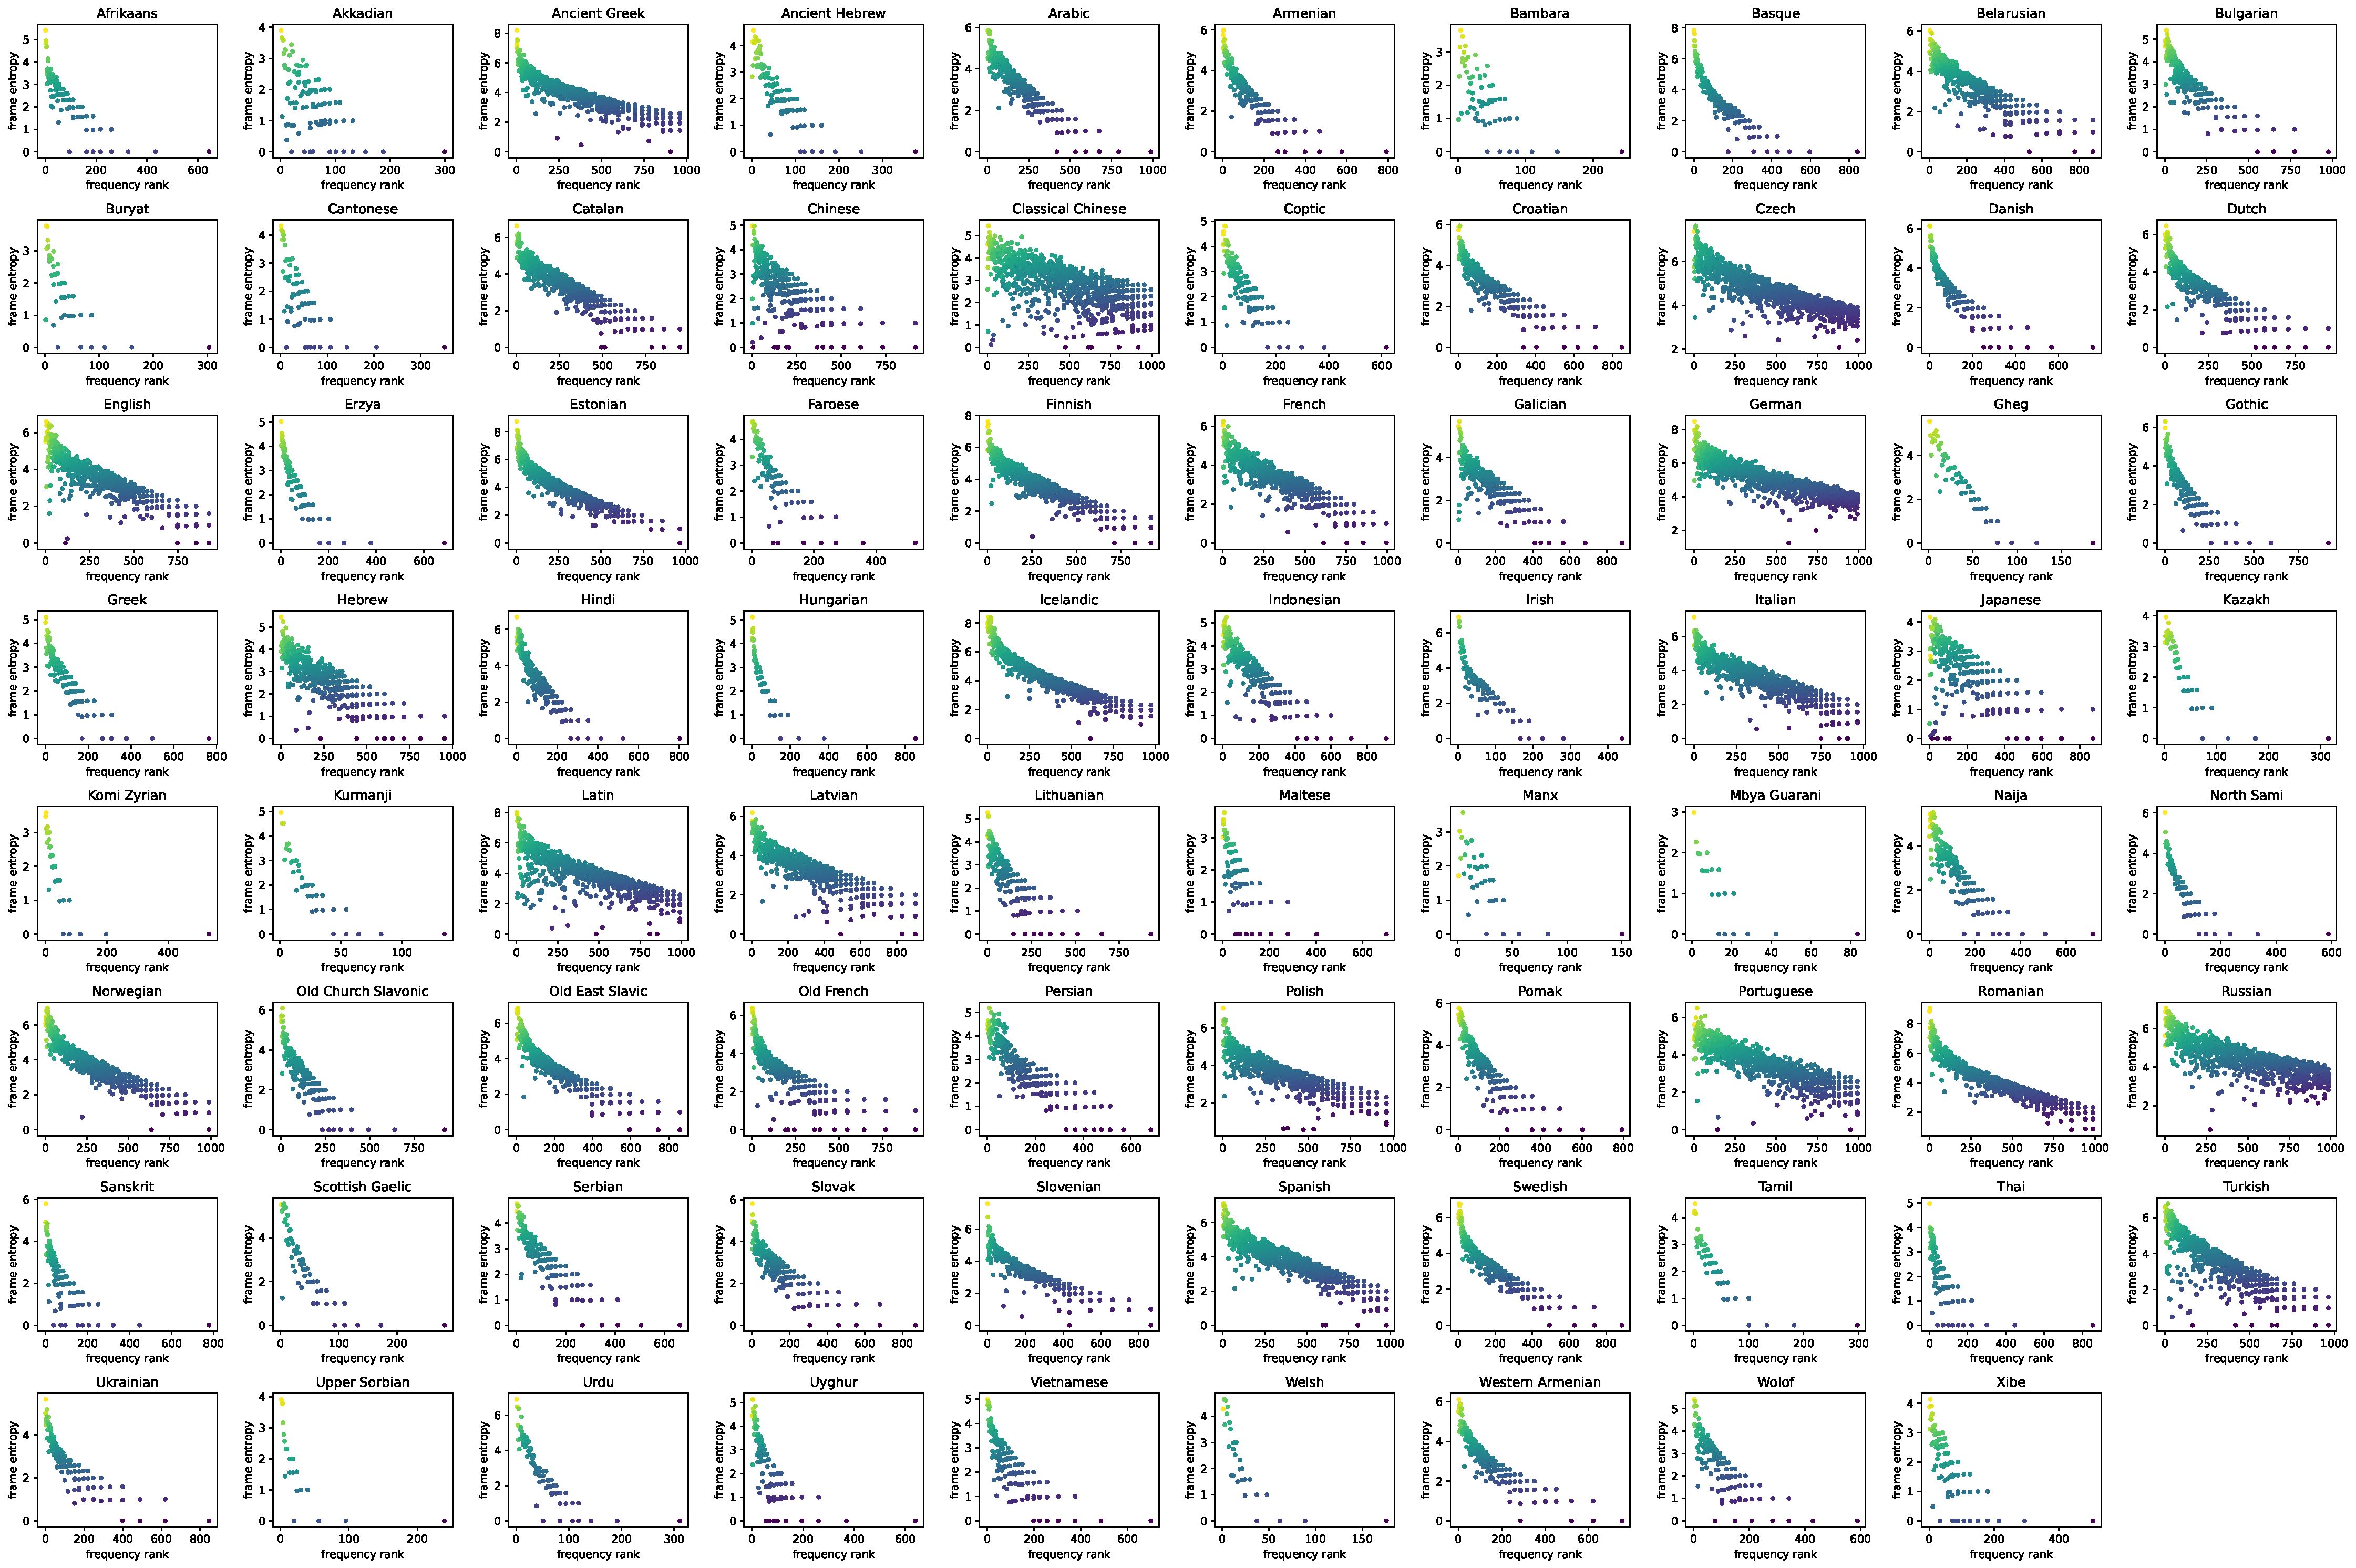
\includegraphics[width=\textwidth]{figures/exp2/joint_entropy_freq.pdf}
  \caption{Scatter plots showing relationship between valency frame entropy and frequency rank of verbs, color shows number of frames associated with the verb (yellow = higher, blue = lower)}
  \label{fig:joint_entropy_freq}
\end{sidewaysfigure}

Spearman's rank correlation results show robust correlation between frequency and valency frame entropy. I include again only languages with at least 50 verbs for which valid entropy measures can be calculated. Strong to very strong correlations (defined as $\rho\geq.70$, following \citealp{schober2018}) are observed in 48 out of 59 languages and moderate correlations ($\rho\geq.40$) are observed in 58 out of 59 languages, with Japanese being the only exception.  The mean $\rho$ value is 0.78, with a standard deviation of 0.14.

Subsampling results help guard against possible circularity by using the same sample size for each verb, at the expense of possibly underestimating entropy for more frequent verbs in particular. One further language (Mbya Guarani) is excluded from subsampling results due to data sparsity. As expected, subsampling results in decreased correlation strength, but 50 out of 59 languages still show moderate correlation strength. The mean $\rho$ value is 0.53, with a standard deviation of 0.14. That the standard deviation remains almost the same indicates that subsampling has a relatively uniform impact across the languages.

Full correlation results are shown in Appendix~\ref{appendix:exp2-rho-freq-valency}. Scatter plots using subsampling results per verb are shown in Fig.~\ref{fig:joint_entropy_freq_subsample}. For some languages, the leveling effect of the subsampling is more visible for higher frequency verbs (e.g. Czech, Romanian), whereas for others, the effect is more uniform across frequencies (e.g. Russian, German).

\begin{sidewaysfigure}[ht]
  \centering
  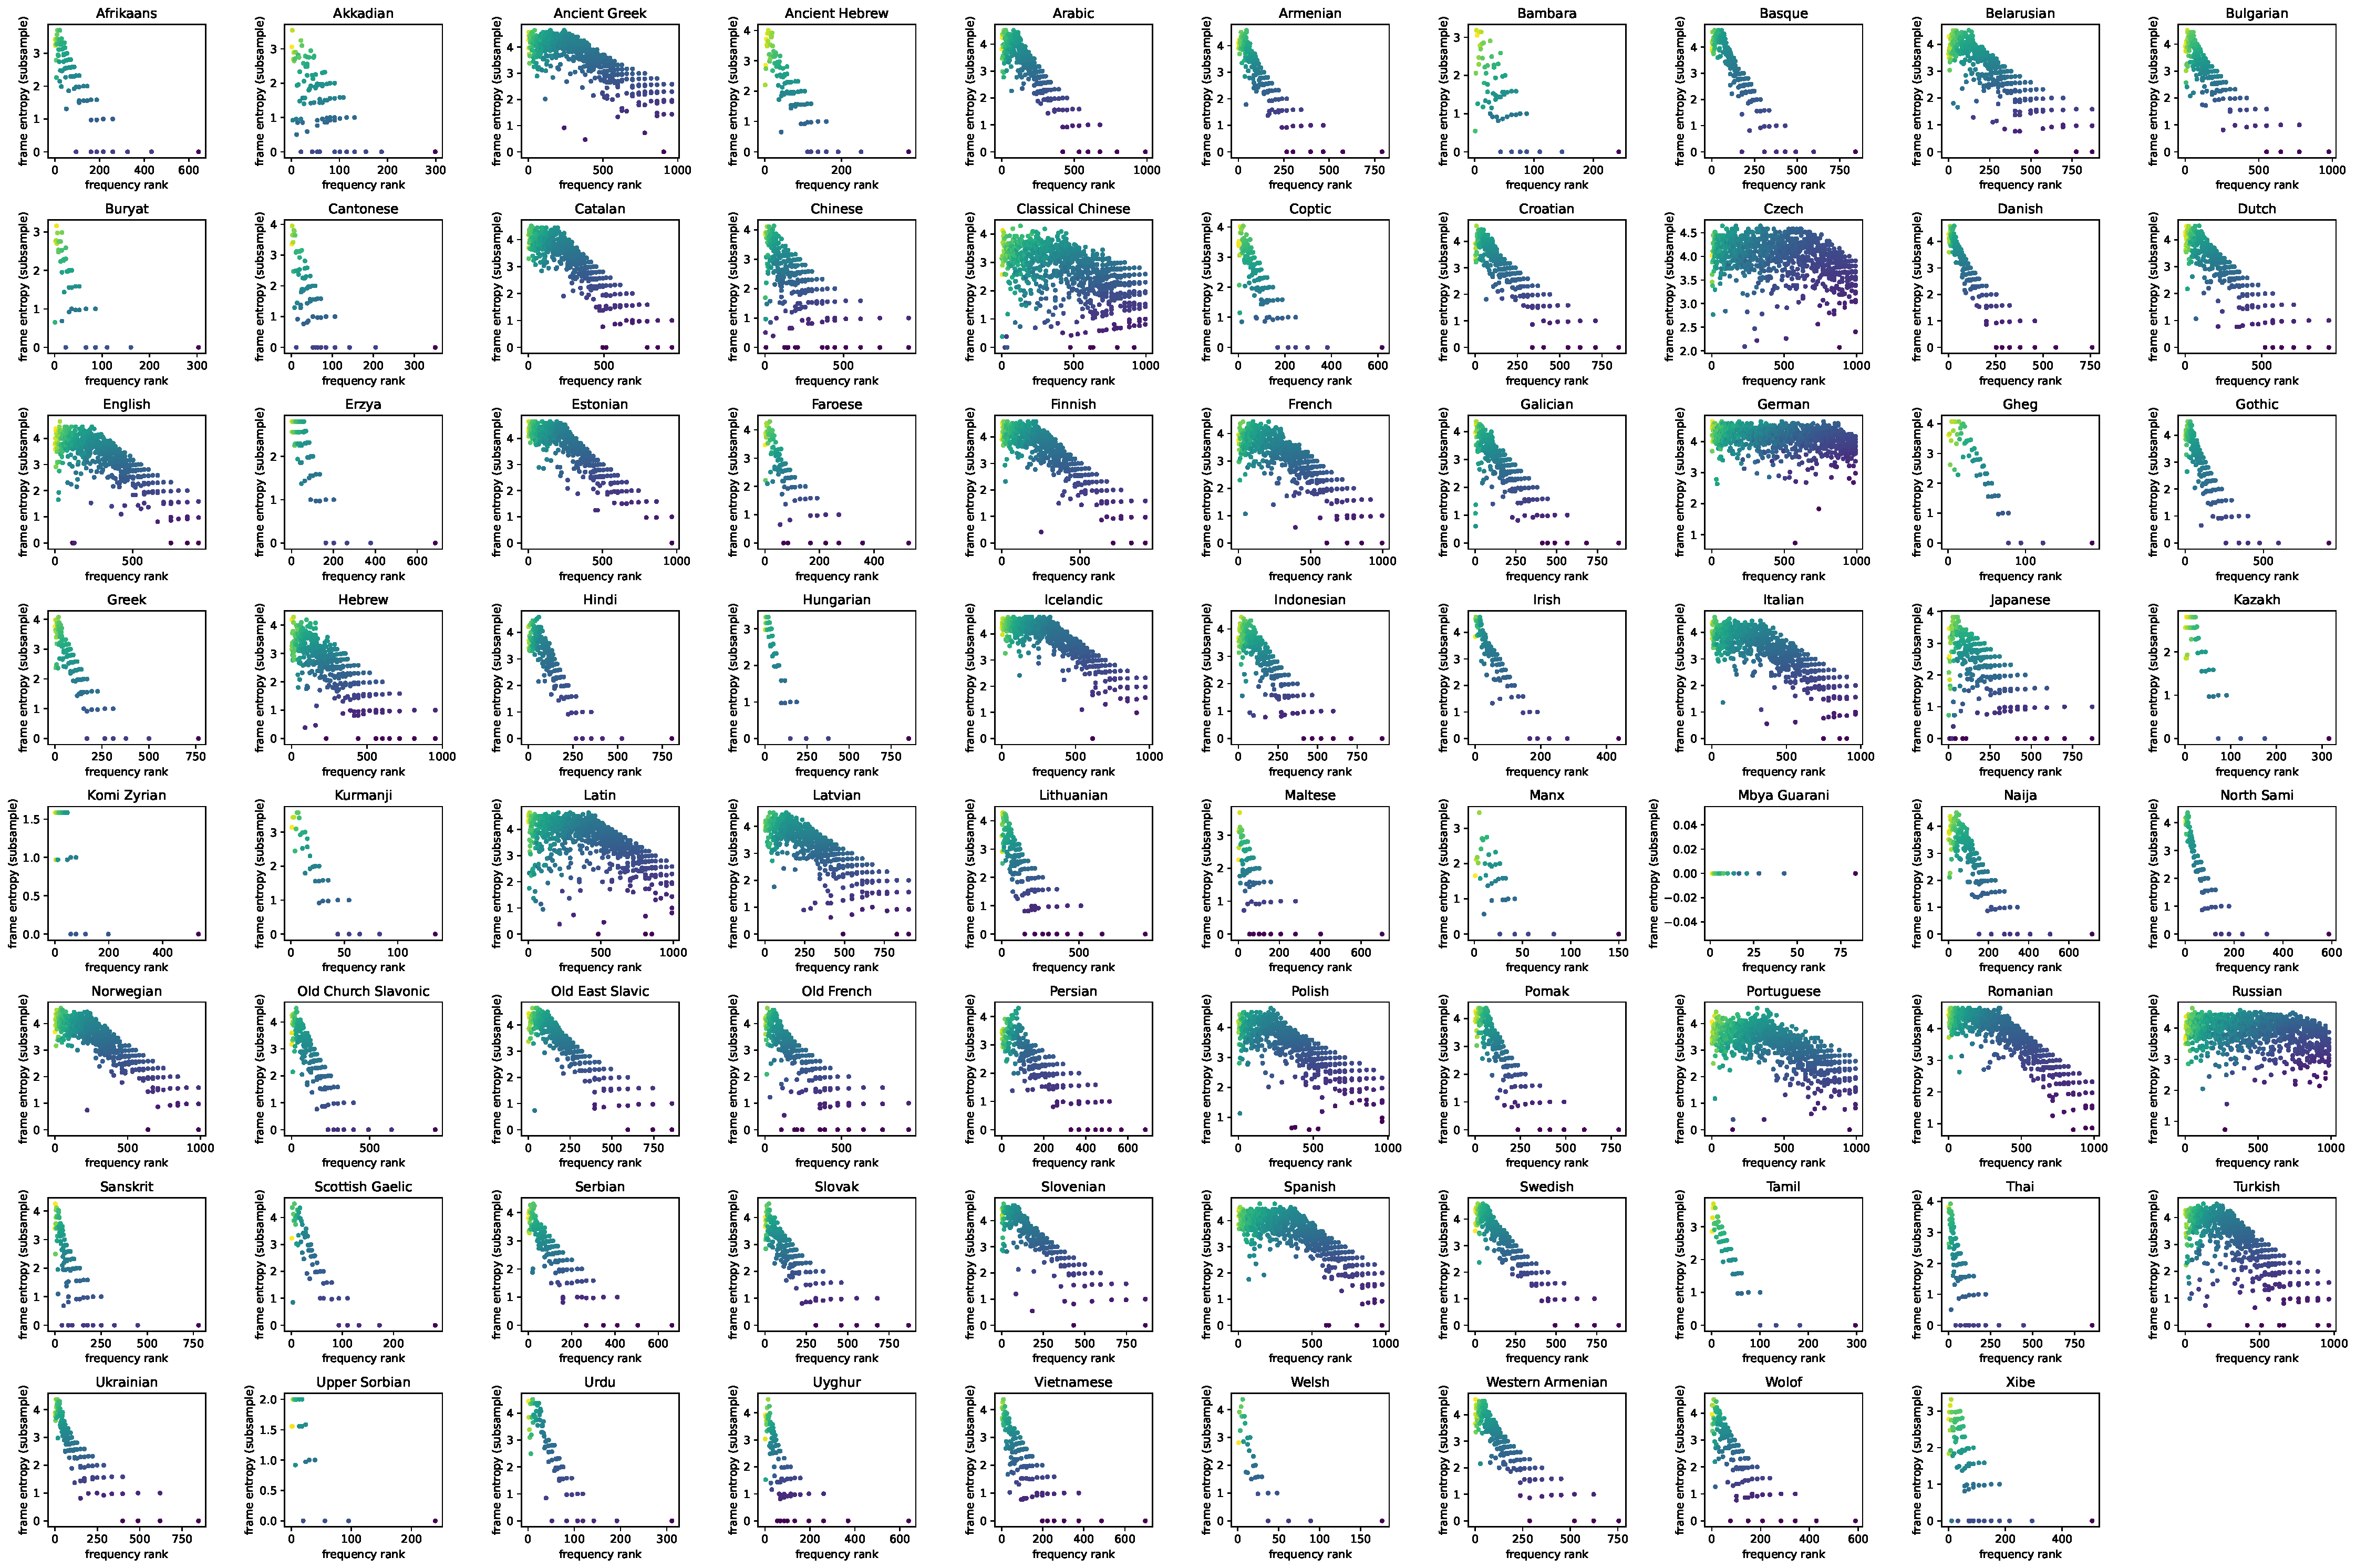
\includegraphics[width=\textwidth]{figures/exp2/joint_entropy_freq_subsample.pdf}
  \caption{Scatter plots showing relationship between valency frame entropy as estimated from the subsample and frequency rank of verbs, color shows number of frames associated with the verb}
  \label{fig:joint_entropy_freq_subsample}
\end{sidewaysfigure}

As can be observed from the scatter plots, the number of frames also shows a strong correlation with verb frequency. In fact, in all the 59 languages studied, the number of frames is more strongly correlated with frequency than valency frame entropy does. This is, however, not to be taken as evidence that the number of frames is a better metric for valency than the valency entropy, because it does not take into account how often the verb appears with a certain valency frame. The high correlation between number of frames and verb frequency may also be taken to indicate that the number of frames are more prone to being affected by the number of observations made hence being a mere proxy of the frequency. While a correlation is indeed expected between frequency and metrics of the valency frame alternation, it stands to reason that more factors, in particular semantics, may affect it as well. A future study with a careful consideration of other factors and using mixed effect models may be better able to explain the results.

Overall, the results strongly support my hypothesis of a positive correlation between a verb's frequency and the valency frame entropy as conditioned on it. It is evidence in support of features of language and lexical structure being shaped by learnability, efficiency and other pressures derived from the communicative function, further bolstered by the cross-lingual applicability of the results. 

However, this does not absolve the need for further investigations, in particular due to the variation in correlation strength between different languages. Several reasons may cause this, all of which require further investigative work either into the UD annotation practices for specific languages or into other aspects of grammar and lexicon. 

One possibility is that the UD annotation schema does not sufficiently account for cross-linguistic differences in argument encoding, or the grammatical categories as designed by UD are not well suited to that languages. This is not unrelated to the second possibility, that because the valency structures of a language interacts with other aspects of grammar, taking further factors into account may be necessary.

An example of this can be seen in the case of Chinese: many of the verbs that are the outliers in terms of being high frequency but having relatively lower entropy are from the category often termed coverbs, e.g., 自 `from', 隨 `follow / with', as their role in the lexicon straddles prepositions and verbs in English. They often serve semantic functions similar to prepositions while behave syntactically as a verb. As their semantic function are relatively narrow, however, so do they only appear much fewer valency frames than other verbs of similar frequency does. Such examples bring into question how strict the boundaries of word categories should be and a fuller picture of valency may well need to better situate the verb category within the overall lexicon.

% % correlation between frequency and dependency relation entropy

% As an additional test, we also confirm that individual dependency relations do not correlate with frequency. This is as expected and confirms the validity of valency frame as a suitable level for analyzing argument structure.


\section{Experiment 3: Word order or case? Cross-lingual variation in valency encoding strategies}\label{sec:exp3-ablation}
\subsection{Introduction}

Typological differences regarding word order and case marking necessarily means that different languages will have to use different strategies for encoding valency frames. On the one hand, it is a straightforward matter that a language cannot use case marking to encode a valency frame if it does not have case marking and a language with more flexible word order is less likely to use word order to encode its valency frame. On the other hand, the trade-off between word order and case marking in languages has been a well-studied topic in typology, which naturally begets the question if such a trade-off can be observed in how languages encode their valency frames.

This experiment examines the cross-lingual variation in valency encoding strategies by testing two hypotheses. The first a relatively simple hypothesis, simply that languages use word order and case marking to encode valency information. The operationalized prediction is that the correlation between valency frame entropy and verb frequency confirmed in Experiment 2 should be weaker, if the valency frame encoding leaves out either word order information, case marking, or both. An ablation study will seek to confirm it.

The second hypothesis uses conditional entropy to quantify the contribution of word order and case marking information to entropy. If the trade-off does 

\subsection{Methodology}

The valency encoding information is split into three sets of variables, with one set each storing information about dependency relation presence $X_1,\ldots,X_n$, relative word order $Y_1,\ldots,Y_n$, and case marking $Z_1,\ldots,Z_n$, with the subscript number representing a UD argument slot (e.g. *nsubj*, *obj*, ...) and with images $\mathcal{X}_{1},\ldots,\mathcal{X}_{n}$,  $\mathcal{Y}_{1},\ldots,\mathcal{Y}_{n}$, $\mathcal{Z}_{1},\ldots,\mathcal{Z}_{n}$ and variable $V$ representing a verb in the lexicon $\mathcal{V}$. The full valency frame entropy as calculated in Experiment 2 is now represented as 

\begin{equation*}
  \begin{split}
   & H_{joint}(X_1,\ldots,X_{n},Y_1,\ldots,Y_{n},Z_1,\ldots,Z_n|V=v) \\
  =& -\sum\limits_{x_1\in{}\mathcal{X}_1}\cdots\sum\limits_{x_n\in{}\mathcal{X}_n}\sum\limits_{y_1\in{}\mathcal{Y}_1}\cdots\sum\limits_{y_n\in{}\mathcal{Y}_n}\sum\limits_{z_1\in{}\mathcal{Z}_1}\cdots\sum\limits_{z_n\in{}\mathcal{Z}_n}\\
  &{P(x_1,\ldots,x_{n}, y_1,\ldots,y_{n}, z_1,\ldots,z_{n}|V=v)\log_2P(x_1,\ldots,x_{n}, y_1,\ldots,y_{n}, z_1,\ldots,z_{n}|V=v)}
  \end{split}
\end{equation*}

For the correlation strength comparison, we calculate (1) valency frame entropy without word order information; (2) valency frame entropy without case marking information; and (3) valency frame entropy without word order and without case marking information. Spearman's rank correlation is then calculated between verb frequency and each of the three post-ablation valency measures.

The conditional entropy is calculated using the chain rule by subtracting the entropy of all other variables from the full entropy. For example, the conditional entropy of word order information will be calculated by subtracting the entropy of presence and case marking variables from the full valency entropy:

\begin{equation*}
  \begin{split}
   & H_{joint}(Y_1,\ldots,Y_{n}| V = v, X_1,\ldots,X_{n},Z_1,\ldots,Z_n)\\
  =&H_{joint}(X_1,\ldots,X_{n},Y_1,\ldots,Y_{n},Z_1,\ldots,Z_{n}|V=v)  \\
  &- H_{joint}(X_1,\ldots,X_{n},Z_1,\ldots,Z_{n}|V=v)
  \end{split}
\end{equation*}

and likewise for the conditional entropy of case marking. The conditional entropy can be intuitively understood as the unique contribution of the variables towards the full entropy, not predictable from other variables. It can also be understood as the entropy of this variable minus mutual information shared with other variable. Conditional measures are then aggregated at a language level for cross-lingual comparison.

\subsection{Results and analysis}

% correlation strength comparison

Lower correlation strength are observed


% conditional entropy as percentage of the full entropy 
Delta between them 


\section{Experiment 4: Frequency correlation with verb entropy}\label{sec:exp4-verb-entropy}

\subsection{Introduction}

So far the experiments have focused on calculating the valency frame entropy conditioned on verb choice. While this does not necessitate the lexeme-based view of valency, lexeme is still the level at which experiments are performed and analysis made. As the hypotheses themselves are motivated by constraints on language structure that derive from its communicative function, they should nevertheless be neutral with respect to which theory of valency one subscribes to. 

Consequently, if one were to adopt the frame-based view of valency and insist on using the frame as the level of analysis, a symmetric hypothesis can be made: namely that given a new metric of verb entropy conditioned on valency frame, we would see a similar frequency effect where the entropy of lexical choice would correlate with the frequency of the valency frame. 

This experiment undertakes to examine exactly that hypothesis and verify the expected symmetry.

\subsection{Methodology}

Given the same variable definitions as in experiment 2, the entropy value for the verb given a single slot is defined as

\begin{equation*}
  \begin{split}
   & H(V|X_1=x_1,\ldots,X_n=x_n)  \\
  =&-\sum\limits_{v\in{}\mathcal{V}}{P(V=v|X_1=x_1,\ldots,X_n=x_n)\log_2P(V=v|X_1=x_1,\ldots,X_n=x_n)}
  \end{split}
\end{equation*}

Here, $P(V=v|X_1=x_1,\ldots,X_n=x_n)$ represents the conditional probability of the outcome that the verb $v$ from the vocabulary $\mathcal{V}$ is selected for the verb slot $V$ given an already determined valency frame $X_1=x_1,\ldots,X_n=x_n$. The entropy of $V$ is calculated by summing the products of these probabilities with their logarithms (base 2) taken, each corresponding to a possible outcome $v_k$.

The rest of the experiment is similarly done in symmetry to experiment 2. Spearman's rank correlation will be calculated with valency frame frequency on the one hand and verb entropy conditioned on the valency frame on the other. 

\subsection{Results and analysis}

The results are as expected.


% \section{Experiment 4: Verb specificity and the argument-adjunct distinction}\label{sec:exp4-verb-specificity}

% \subsection{Introduction}

% Let us reexamine the argument-adjunct distinction in argument structure again. This distinction is relevant to syntax and semantics at a sentential level and usually formulated to state that the former is obligatory to complete the meaning of the verb, and the latter not. As it is concerned with morphosyntax first and foremost, this study focuses on the syntactic observation of \textit{verb specificity} \citep[cf.]{haspelmath2015a}, namely that verbs are more selective with regard to arguments but can be more freely used with adjuncts. 

% This experiment seeks to quantify the verb specificity by looking at the variance of dependency relation entropy when conditioned the verb. The entropy measures the average surprisal associated with this relation (including presence, word order and case marking) when given the verb. If a verb never or always appears with a certain dependency relation with a certain word order and case marking, the entropy of this dependency relation conditioned on the verb will be 0; the opposite scenario, where a verb is equally likely to appear with or without certain dependency frame, would result in the highest possible entropy. The specific ceiling value is dependent upon the possible `frames' of this entropy given the number of case marking and word order flexibility and will vary by language.

% Recall the bimodal distribution of transitive verbs observed \subsection{subsec:transitivity-lexicon}, verbs that are highly transitive or highly intransitive will have high entropy, carrier more information. Verb specific feature leads to higher entropy.


% The less verb specific a dependency is, the more uniform it will be between verbs resulting in lower entropy in general. This is on an entropy per dependency relation level.

% \subsection{Methodology}

% $$H(X_{k} | V = v, X_{1},\cdots,X_{n} \setminus X_{k}) = H( V = v, X_{1},\cdots,X_{n}) - H( V = v, X_{1},\cdots,X_{n}\setminus X_{k})$$

% \subsection{Results and analysis}

\chapter{Conclusion and outlook}\label{chapter:conclusion}

As indicated by the title, this thesis reports on several experiments on the cross-linguistic patterns in verbal valency systems. The exploratory nature of the experiments and the range of experiments make it easy to lose track of the overarching research questions. I summarize the experiments and their findings in this section, and discuss them in conjunction to how they help answer these questions. 

The two main research questions of the thesis are: (1) Do quantitative methods provide a way to characterize verbal valency and verbal valency systems in a manner that facilitates cross-lingual comparison? (2) If so, do the results allow us to draw inferences about cross-lingual differences as well as commonalities in how languages structure their verbal valency systems.

Two substantive experiments (1-2) are presented that address both research questions from different perspectives. Two additional experiments (3-4) point to possible future directions of work. 

Experiment 1 starts with a more basic measure for one aspect of valency, i.e. transitivity. Using corpus-based and quantitative versions of the transitivity ratio metric, it shows a general but not inviolable common tendency of languages to structure their verbal lexicon towards both ends of the transitivity spectrum, and show that the metric indicates areal and genetic patterns of transitivity between languages. Experiment 2-4 expands the scope of investigation and use information-theoretic metrics of valency frame entropy as a more holistic characterization of verbal valency. Correspondingly, linguistic differences and universals are explored with hypotheses motivated by cognitive linguistics approaches, taking learnability and efficiency constraints on language structure into account.

The results from the experiments support the view that how languages organize their verbal valency systems as well as the parts of verbal lexicon and grammar that are relevant shares cross-linguistic similarities shaped by common constraints but also shows differences in the different strategies they employ. It is relatively neutral in terms of lexeme- vs. frame-based view of valency but results from experiment 4 also suggests that the two views may not be irreconcilable with different languages leveraging different parts of the grammar to achieve the same communicative goals.

\section{Note on reproducibility}
Code and results for the thesis will be made available at the following repository: \url{https://github.com/siyutao/verbal-valency-ud}


\appendix
\chapter{Experiment 1 Results}
\section{Per language transitivity statistics}
\begin{longtable}{lrrrr}
    \toprule
    language name & total & tr verb percent & 4 mean & 4 weighted mean \\
    \midrule
    \endfirsthead
    \toprule
    language name & total & tr verb percent & 4 mean & 4 weighted mean \\
    \midrule
    \endhead
    \midrule
    \multicolumn{5}{r}{Continued on next page} \\
    \midrule
    \endfoot
    \bottomrule
    \endlastfoot
    Akkadian & 45 & 62.22\% & 73.38\% & 80.32\% \\
    Armenian & 227 & 70.48\% & 51.53\% & 48.98\% \\
    Welsh & 17 & 70.59\% & 35.53\% & 9.45\% \\
    Gheg & 50 & 86.00\% & 65.95\% & 64.82\% \\
    Norwegian & 765 & 89.67\% & 48.30\% & 44.80\% \\
    Old East Slavic & 500 & 65.80\% & 55.43\% & 48.87\% \\
    English & 771 & 88.72\% & 55.51\% & 52.90\% \\
    French & 733 & 90.86\% & 55.15\% & 51.29\% \\
    Slovenian & 514 & 79.57\% & 64.30\% & 55.55\% \\
    Hebrew & 531 & 51.98\% & 35.94\% & 33.50\% \\
    Kurmanji & 21 & 52.38\% & 27.94\% & 38.02\% \\
    Italian & 921 & 82.41\% & 55.70\% & 54.50\% \\
    Turkish & 773 & 73.74\% & 47.20\% & 48.54\% \\
    Finnish & 682 & 69.94\% & 53.94\% & 48.41\% \\
    Indonesian & 330 & 91.21\% & 49.74\% & 51.21\% \\
    Ukrainian & 228 & 66.23\% & 50.64\% & 45.33\% \\
    Dutch & 497 & 75.65\% & 38.10\% & 37.51\% \\
    Polish & 1059 & 61.95\% & 47.67\% & 34.07\% \\
    Portuguese & 1203 & 77.47\% & 52.46\% & 52.45\% \\
    Kazakh & 30 & 63.33\% & 45.43\% & 39.91\% \\
    Latin & 1143 & 72.35\% & 44.50\% & 40.85\% \\
    Old French & 422 & 70.14\% & 52.96\% & 53.50\% \\
    Spanish & 941 & 92.88\% & 65.36\% & 61.08\% \\
    Buryat & 27 & 51.85\% & 35.67\% & 36.83\% \\
    Icelandic & 997 & 86.56\% & 51.81\% & 41.05\% \\
    Estonian & 672 & 67.71\% & 53.48\% & 49.69\% \\
    Croatian & 386 & 84.97\% & 58.34\% & 50.27\% \\
    Gothic & 195 & 58.46\% & 50.92\% & 45.80\% \\
    North Sami & 75 & 76.00\% & 49.35\% & 37.91\% \\
    Naija & 200 & 88.50\% & 54.92\% & 45.43\% \\
    German & 1998 & 89.69\% & 57.18\% & 56.84\% \\
    Latvian & 787 & 63.79\% & 45.18\% & 37.71\% \\
    Chinese & 369 & 83.74\% & 60.56\% & 62.90\% \\
    Irish & 107 & 77.57\% & 54.22\% & 30.87\% \\
    Xibe & 62 & 70.97\% & 65.22\% & 58.37\% \\
    Bambara & 50 & 62.00\% & 54.14\% & 43.08\% \\
    Lithuanian & 212 & 58.02\% & 44.38\% & 41.48\% \\
    Galician & 339 & 88.79\% & 71.14\% & 70.44\% \\
    Vietnamese & 150 & 84.00\% & 62.00\% & 64.25\% \\
    Greek & 145 & 77.24\% & 50.65\% & 48.68\% \\
    Catalan & 627 & 98.25\% & 81.12\% & 75.86\% \\
    Swedish & 391 & 86.45\% & 47.79\% & 46.49\% \\
    Russian & 2558 & 59.34\% & 43.43\% & 37.35\% \\
    Czech & 2083 & 72.88\% & 54.72\% & 46.76\% \\
    Erzya & 87 & 54.02\% & 40.36\% & 36.01\% \\
    Thai & 69 & 69.57\% & 51.99\% & 63.16\% \\
    Basque & 249 & 78.71\% & 56.54\% & 54.51\% \\
    Slovak & 279 & 55.91\% & 44.26\% & 42.32\% \\
    Tamil & 41 & 80.49\% & 50.32\% & 42.73\% \\
    Maltese & 67 & 43.28\% & 30.35\% & 27.34\% \\
    Ancient Greek & 1111 & 81.55\% & 60.97\% & 58.47\% \\
    Ancient Hebrew & 89 & 73.03\% & 53.43\% & 48.40\% \\
    Mbya Guarani & 5 & 60.00\% & 57.33\% & 51.46\% \\
    Urdu & 69 & 85.51\% & 62.27\% & 65.23\% \\
    Romanian & 1002 & 79.84\% & 48.65\% & 48.86\% \\
    Persian & 308 & 72.73\% & 54.05\% & 50.27\% \\
    Japanese & 381 & 61.15\% & 50.06\% & 33.54\% \\
    Hungarian & 73 & 60.27\% & 44.39\% & 40.16\% \\
    Hindi & 202 & 83.66\% & 61.24\% & 60.74\% \\
    Classical Chinese & 1166 & 79.42\% & 60.76\% & 63.84\% \\
    Faroese & 114 & 71.93\% & 40.13\% & 32.51\% \\
    Sanskrit & 106 & 74.53\% & 57.49\% & 51.74\% \\
    Arabic & 407 & 72.48\% & 46.74\% & 39.65\% \\
    Wolof & 155 & 87.10\% & 55.11\% & 53.52\% \\
    Bulgarian & 348 & 81.32\% & 47.10\% & 47.64\% \\
    Cantonese & 45 & 73.33\% & 55.92\% & 50.99\% \\
    Pomak & 229 & 72.49\% & 63.20\% & 61.76\% \\
    Old Church Slavonic & 211 & 54.50\% & 46.60\% & 43.49\% \\
    Upper Sorbian & 10 & 70.00\% & 40.82\% & 38.59\% \\
    Danish & 212 & 88.68\% & 54.47\% & 51.92\% \\
    Komi Zyrian & 25 & 32.00\% & 28.64\% & 25.52\% \\
    Manx & 25 & 72.00\% & 47.98\% & 22.92\% \\
    Afrikaans & 117 & 82.91\% & 60.90\% & 65.13\% \\
    Belarusian & 587 & 68.14\% & 49.27\% & 44.41\% \\
    Coptic & 127 & 65.35\% & 41.30\% & 43.55\% \\
    Serbian & 214 & 73.36\% & 47.94\% & 38.45\% \\
    Western Armenian & 299 & 75.92\% & 54.87\% & 50.66\% \\
    Scottish Gaelic & 53 & 77.36\% & 37.74\% & 16.17\% \\
    Uyghur & 80 & 53.75\% & 37.84\% & 32.95\% \\
\end{longtable}
    

\backmatter

% optional: list of figures, list of tables
% \listoffigures
% \listoftables

\chapter{Bibliography}
\printbibliography[heading=none]

\end{document}
